\SourcePage{166}
\SGAchapter{XVII}{固有支撑上同调}{Cohomologie à supports propres}
\begin{center}P. Deligne\footnote{本讲与下一讲写于 1968 年及 1969 年，重述并补充了 A. Grothendieck 于 1964 年春所作的口头报告。撰稿人未曾参加口头讨论班，部分参考了 A. Grothendieck 的笔记。}\end{center}
\textbf{引言。}
本讲展开\Term{proper-support-cohomology}{固有支撑上同调}的\Term{form}{形式}体系。这里相当仔细地处理了变性问题；在口头讨论班中，这些问题只是得到了可信的说明。这也解释了本讲何以如此之长，其中第 1 至第 4 节专论\Term{category}{范畴}与一般\Term{topology}{拓扑}。我们强烈建议读者只读第 5、6 节，
\SourcePage{167}
本讲的几何实质集中在那里（第 5 节：\Term{proper-support-cohomology}{固有支撑上同调}的构造与变性，\Term{base-change}{基变换}、\Term{finiteness}{有限性}、\Term{finite-tor-dimension}{有限 Tor 维数}及\Term{comparison-theorem}{比较定理}；第 6 节：\Term{quasi-finite}{拟有限}\Term{flat}{平坦}\Term{morphism}{态射}的\Term{trace-morphism}{迹态射}理论）。

第 1、2 节“回顾”关于\Term{derived-category}{导出范畴}的一些结果。第 1 节第 1 小节专论\Term{signature}{符号}的\Term{form}{形式}体系。第 3 节处理如何把两套变性\Term{form}{形式}体系\Term{gluing}{粘合}起来的问题。第 4 节引入\Term{flat-resolution}{平坦解消}，并研究 Godement \Term{flasque-resolution}{松弛解消}的特殊性质。

本讲中的高阶\Term{proper-direct-image}{固有支撑直接像}\Term{functor}{函子} $R^qf_!$ 及产生它们的\Term{functor}{函子} $Rf_!$，只对 $f$ 为\Term{compactifiable-morphism}{可紧化态射}（3.2.1）的情形定义。由 B. Saint-Donat 撰写的附录说明，如何把这一定义推广到靶为\Term{quasi-compact}{拟紧}\Term{quasi-separated}{拟分离}的\Term{finite-type}{有限型}\Term{separated}{分离}\Term{morphism}{态射}。

第 5 节第 5 小节（对称积的\Term{cohomology}{上同调}）在本讨论班以后不再使用。它将在 SGA 5 中用于加强 $L$ 函数的有理性定理。

第 6 节第 3 小节（\Term{continuous}{连续}系数的迹理论）在第 XVIII 讲中只会用于\Term{smooth}{光滑}群这一相对容易的情形；对于关心 \Term{poincare-duality}{Poincaré 对偶}定理（整体\Term{duality}{对偶}）并愿意接受一个超越论证的读者，甚至可以完全不读第 6 节第 3 小节以及第 XVIII 讲第 1 节的大部分。

\SGAsection{0}{术语预备}
\textbf{0.1。}放在两组表示某一\Term{category}{范畴}的\Term{object}{对象}的\Term{signature}{符号}之间的等号 $=$，有时（滥用记号地）表示这些\Term{object}{对象}\Term{canonical}{典范}\Term{isomorphism}{同构}。原则上，该\Term{category}{范畴}和该\Term{canonical}{典范}\Term{isomorphism}{同构}都应当已事先定义。在图中，等号这时表示该\Term{isomorphism}{同构}本身。

\textbf{0.2.0。}设 $f:S\to S'$ 为\Term{site}{景}的\Term{morphism}{态射}（第 IV 讲 4.9.3）。若 $U$、$U'$ 分别是 $S$、$S'$ 的\Term{object}{对象}，则从 $U$ 到 $U'$ 的一个 $f$-\Term{morphism}{态射}，按定义就是从 $U$ 到 $f^*U'$ 的\Term{morphism}{态射}。对于\Term{scheme}{概形}的\Term{etale-site}{平展景}，这就回到了通常的概念。

\textbf{0.2.1。}若 $F$、$F'$ 分别是 $S$、$S'$ 上的\Term{sheaf}{层}，则从 $F$ 到 $F'$ 的一个 $f$-\Term{morphism}{态射}，可以\Term{equivalence}{等价}地是：
\begin{enumerate}
\item[(i)] 从 $f^*F'$ 到 $F$ 的\Term{morphism}{态射}；
\item[(ii)] 从 $F'$ 到 $f_*F$ 的\Term{morphism}{态射}；
\end{enumerate}
\SourcePage{168}
\begin{enumerate}
\item[(iii)] 一个函数，它对 $S$ 的\Term{object}{对象} $U$ 到 $S'$ 的\Term{object}{对象} $U'$ 的每个 $f$-\Term{morphism}{态射} $\varphi$，赋予一个从 $F'(U')$ 到 $F(U)$ 的函数，并且与 $\varphi$ 同 $S$ 或 $S'$ 中\Term{arrow}{箭头}的复合相容。\footnote{这些术语与把 $S$ 的\Term{object}{对象}同相应的\Term{adjunction}{伴随}\Term{sheaf}{层}等同的做法并不相容。}
\end{enumerate}
由 (i)、(ii)、(iii) 可见，\Term{set}{集合}\Term{sheaf}{层}在\Term{site}{景}的\Term{category}{范畴}上组成一个\Term{fibered-category}{纤维范畴}，同时也是\Term{cofibered-category}{余纤维范畴}。

\Term{ringed-site}{赋环景}上的左模\Term{sheaf}{层}也一样。\Term{scheme}{概形}上的\Term{etale-sheaf}{平展层}也一样；后者并不能立即看成前述情形的特例，因为\Term{site}{景}实际上组成一个 $2$-\Term{category}{范畴}，而“$X$ 的\Term{etale-site}{平展景}”对 $X$ 只构成一个\Term{pseudofunctor}{伪函子}（第 VII 讲 1.4）。

上述定义使变动的\Term{site}{景}上的\Term{set}{集合}\Term{sheaf}{层}（相应地，……）成为\Term{site}{景}\Term{category}{范畴}上的一个\Term{fibered-category}{纤维范畴}，其\Term{fiber-category}{纤维范畴}是通常的\Term{set}{集合}\Term{sheaf}{层}（相应地，……）\Term{category}{范畴}的\Term{opposite-category}{反范畴}。

\textbf{0.3。}设 $I$ 是\Term{finite}{有限}集，$\varepsilon:I\to\{+1,-1\}$ 是一个函数，$(\mathcal A_i)_{i\in I}$ 是一族由\Term{translation-functor}{平移函子} $T_i$ \Term{graded}{分次}的\Term{additive-category}{加性范畴}（CD I 1.10），$F$ 是从这些 $\mathcal A_i$ 到由\Term{translation-functor}{平移函子} $T$ \Term{graded}{分次}的\Term{additive-category}{加性范畴} $\mathcal A$ 的\Term{multiadditive-functor}{多加性多函子}。假定当 $\varepsilon_i=1$（相应地，$\varepsilon_i=-1$）时，$F$ 关于第 $i$ 个变元\Term{covariant}{协变}（相应地，\Term{contravariant}{反变}）。对 [CD] I 1.1 略作修改和补充，我们称 $F$ 为\Term{graded-functor}{分次函子}，如果给定了一族 $T\circ F$ 与 $F\circ T_i^{\varepsilon_i}$ 之间的\Term{functor}{函子}\Term{isomorphism}{同构} $(\varphi_i)_{i\in I}$，使对于 $I$ 中 $i\ne j$，下图\Term{anticommutative}{反交换}：
\[
\begin{tikzcd}[column sep=large,row sep=large]
F\circ(T_i^{\varepsilon_i},T_j^{\varepsilon_j}) \arrow[r,"\varphi_j*T_i^{\varepsilon_i}"] \arrow[d,"\varphi_i*T_j^{\varepsilon_j}"'] & T\circ F\circ T_i^{\varepsilon_i} \arrow[d,"T*\varphi_i"]\\
T\circ F\circ T_j^{\varepsilon_j} \arrow[r,"T*\varphi_j"'] & T\circ T\circ F
\end{tikzcd}\qquad(-).
\]
两个\Term{graded-functor}{分次函子}的复合如何定义，以及它仍为\Term{graded-functor}{分次函子}的验证，留给读者。

\textbf{0.4。}设 $\mathcal A$ 为\Term{additive-category}{加性范畴}，$I$ 为\Term{finite}{有限}集。对 $i\in I$，以 $1_i$ 表示 $\mathbf Z^I$ 的第 $i$ 个基向量。$\mathcal A$ 的一个 $I$ 重\Term{complex}{复形}（相应地，一个朴素 $I$ 重\Term{complex}{复形}）由以下资料组成：
\begin{enumerate}
\item[(a)] 一族 $\mathcal A$ 的\Term{object}{对象} $(K^k)_{k\in\mathbf Z^I}$；
\item[(b)] 对每个 $i\in I$ 及 $k\in\mathbf Z^I$，一个\Term{arrow}{箭头} $d_i^k:K^k\to K^{k+1_i}$，满足
\[
d_i^{k+1_i}d_i^k=0,\qquad d_i^{k+1_j}d_j^k+d_j^{k+1_i}d_i^k=0\quad(i\ne j)
\]
（相应地，$d_i^{k+1_j}d_j^k=d_j^{k+1_i}d_i^k$）。
\end{enumerate}

\SourcePage{169}
\textbf{0.5。}我们称\Term{category}{范畴} $\mathcal C$ 的一个\Term{pro-object}{pro-对象}，是一个从 $\mathcal C$ 到 $(\mathrm{Ens})$ 的\Term{functor}{函子}，它是\Term{representable-functor}{可表函子}的\Term{filtered-colimit}{滤过归纳极限}（沿某个小\Term{filtered-category}{滤过范畴}）（参见第 I 讲 8.10）。每个\Term{pro-object}{pro-对象}都是沿某个小的\Term{filtered-ordered-set}{滤过有序集}的\Term{representable-functor}{可表函子}的\Term{colimit}{归纳极限}。若 $X_i$ 是由某个小\Term{filtered-category}{滤过范畴}标定的 $\mathcal C$ 的\Term{object}{对象}的\Term{projective-system}{投射系}，则以 $\text{“}\varprojlim\text{”}X_i$ 表示\Term{pro-object}{pro-对象} $\varinjlim h_{X_i}$。

\textbf{0.6。}读者可将 0.5 \Term{dualizing}{对偶化}到\Term{ind-object}{ind-对象}的情形（参见第 I 讲 8.2）。

\textbf{0.7。}依照新术语，以前称为\Term{prescheme}{预概形}的，现在称为\Term{scheme}{概形}；以前称为\Term{scheme}{概形}的，现在称为\Term{separated}{分离}\Term{scheme}{概形}。

\textbf{0.8。}\Term{ringed-scheme}{赋环概形}的\Term{category}{范畴}，其\Term{object}{对象}是那些在其\Term{etale-site}{平展景}上给定了环\Term{sheaf}{层}的\Term{scheme}{概形}；从 $(S,\mathcal A)$ 到 $(T,\mathcal B)$ 的\Term{arrow}{箭头}是一个二元组，由\Term{scheme}{概形}\Term{morphism}{态射} $f:S\to T$ 和环\Term{sheaf}{层}的\Term{homomorphism}{同态} $\varphi:f^*\mathcal B\to\mathcal A$ 组成。称\Term{scheme}{概形}\Term{morphism}{态射} $f$ 由 $(f,\varphi)$ 诱导。

\textbf{0.9。}若 $X$ 是 $Y$ 上的\Term{scheme}{概形}，则以 $(X/Y)^n$ 表示 $X$ 在 $Y$ 上的 $n$ 重\Term{fiber-product}{纤维积}。

\textbf{0.10。}设 $S$ 是\Term{scheme}{概形}。称配备\Term{etale-topology}{平展拓扑}（相应地，fppf、\Term{fpqc-topology}{fpqc 拓扑}）的\Term{site}{景} $\mathrm{Sch}_{/S}$ 为 $S$ 的大\Term{etale-site}{平展景}（相应地，大 fppf \Term{site}{景}、大 fpqc \Term{site}{景}）（SGA 3 第 IV 讲 6.3）。应当注意，它不是一个 $\mathcal U$-\Term{site}{景}（$\mathcal U$ 是\Term{finite}{有限}的\Term{universe}{宇宙}，$\mathrm{Sch}_{/S}$ 由属于 $\mathcal U$ 的\Term{scheme}{概形}组成）。

称 $S$ 上的\Term{flat}{平坦}\Term{scheme}{概形}（相应地，\Term{finite-presentation}{有限表现}的\Term{flat}{平坦}\Term{scheme}{概形}）所成的\Term{site}{景}，配备 fpqc（相应地，fppf）\Term{topology}{拓扑}，称为 $S$ 的小 fpqc \Term{site}{景}（相应地，小 fppf \Term{site}{景}）。需要避免混淆时，将\Term{site}{景} $S_{\text{ét}}$（第 VII 讲 1.2）称为 $S$ 的小\Term{etale-site}{平展景}。

\textbf{0.11。}许多地方本应说\Term{site}{景}\Term{morphism}{态射}构成的图本质交换，即在\Term{isomorphism}{同构}意义下交换（参见第 IV 讲 3.2.2），撰稿人却径直说它们是\Term{commutative-diagram}{交换图}。读者可以核实，我们给出的论证同样适用于一般情形。

\textbf{0.12。}A. Grothendieck 在一些地方悄悄引入了“\Term{coherent-scheme}{凝聚概形}”这一术语，以表示“\Term{quasi-compact}{拟紧}\Term{quasi-separated}{拟分离}\Term{scheme}{概形}”。

\textbf{0.13。}若\Term{scheme}{概形} $S$ 上的一个\Term{torsion-sheaf}{挠层} $F$ 是其被 $S$ 上\Term{invertible}{可逆}的整数 $n$ 所消去的子\Term{sheaf}{层}的\Term{colimit}{归纳极限}，则称它与 $S$ 的\Term{residue-characteristic}{剩余特征}互素。

\SGAsection{1}{导出范畴}
\textbf{1.1。\Term{exact-functor}{正合函子}（\Term{signature}{符号}规则）。}
\SourcePage{170}
\textbf{1.1.1。}关于\Term{derived-category}{导出范畴}的基本定理，请参阅 Verdier [9] 及 [2]。本小节特别注意\Term{signature}{符号}问题。

回顾如下：若 $f:X\to Y$ 是\Term{complex}{复形}的\Term{morphism}{态射}（在某个\Term{additive-category}{加性范畴}中；下文均默认如此），则它的\Term{mapping-cone}{锥} $C(f)$ 定义为
\[
C(f)^n=X^{n+1}\oplus Y^n,\qquad d^n=-d_X^{n+1}+f^{n+1}+d_Y^n.\tag{1.1.1.1}
\]
当 $X=0$（相应地，$Y=0$）时，有 $C(f)=Y$（相应地，$C(f)=X[1]$），因此\Term{commutative-diagram}{交换图}
\[
\begin{tikzcd}
0\arrow[r,equal]\arrow[d]&0\arrow[r,equal]\arrow[d]&X\arrow[r,equal]\arrow[d,"f"]&X\arrow[d]\\
X\arrow[r,"f"']&Y\arrow[r,equal]&Y\arrow[r]&0
\end{tikzcd}
\]
定义一个“三角”
\[
X\xrightarrow{f}Y\longrightarrow C(f)\xrightarrow{j}X[1].
\]
在\Term{homotopy-category}{同伦范畴}中，称一个三角为\Term{distinguished-triangle}{区别三角}，如果它\Term{isomorphism}{同构}于这种\Term{form}{形式}的三角；若把其\Term{arrow}{箭头}都变号后成为\Term{distinguished-triangle}{区别三角}，则称其为\Term{antidistinguished-triangle}{反区别三角}。可以验证，逐次\Term{splitting}{分裂}的\Term{complex}{复形}\Term{exact-sequence}{正合列}所定义的三角（[9] 第 10 页，参见 1.1.5.4 的证明）是\Term{antidistinguished-triangle}{反区别三角}，并且在\Term{isomorphism}{同构}意义下，每个\Term{antidistinguished-triangle}{反区别三角}都由此得到。

\textbf{*1.1.2。}利用下列“\Term{form}{形式}规则”，\Term{signature}{符号}计算最为方便。把 $C(f)^n$ 的元素写成 $1\otimes x+y$（$x\in X^{n+1}$，$y\in Y^n$），其中 $1$ 是一个\Term{dimension}{维数}为 $1$ 的“胞腔”，并约定 $d(1)\otimes x=f(x)$。于是
\[
d(1\otimes x+y)=d1\otimes x-1\otimes dx+dy=-1\otimes dx+f(x)+dy.\quad *
\]

\begin{SGAresult}{定义}{1.1.3}
\begin{enumerate}
\item[(i)] 从\Term{triangulated-category}{三角范畴} $\mathcal A$ 到\Term{triangulated-category}{三角范畴} $\mathcal B$ 的\Term{graded-functor}{分次函子}（0.3），若把\Term{distinguished-triangle}{区别三角}变成\Term{distinguished-triangle}{区别三角}，则称为\Term{exact-functor}{正合函子}。
\item[(ii)] 从\Term{triangulated-category}{三角范畴} $\mathcal A$ 到\Term{triangulated-category}{三角范畴} $\mathcal B$ 的\Term{contravariant}{反变}\Term{graded-functor}{分次函子}称为\Term{exact-functor}{正合函子}，如果对 $\mathcal A$ 的每个\Term{distinguished-triangle}{区别三角} $(X,Y,Z,u,v,w)$，三角
\[
(F(Z),F(Y),F(X),F(v),F(u),TF(w))
\]
都是\Term{distinguished-triangle}{区别三角}（此定义中，借助 $F$ 的\Term{graded}{分次}把 $FX$ 与 $TFTX$ 等同）。
\item[(iii)] 设 $(\mathcal A_i)_{i\in I}$ 是\Term{finite}{有限}族\Term{triangulated-category}{三角范畴}，$\varepsilon:I\to\{+1,-1\}$ 是一个函数，$\mathcal A$ 为\Term{triangulated-category}{三角范畴}。从这些 $\mathcal A_i$ 的积到 $\mathcal A$ 的\Term{graded-functor}{分次函子} $F$，在 $\varepsilon(i)=1$ 的变元上\Term{covariant}{协变}，在 $\varepsilon(i)=-1$ 的变元上\Term{contravariant}{反变}；若对于每个 $i\in I$，固定除第 $i$ 个以外的全部变元所得的从 $\mathcal A_i$ 到 $\mathcal A$ 的\Term{functor}{函子}均为\Term{exact-functor}{正合函子}，则称 $F$ \Term{exact-functor}{正合}。
\end{enumerate}
\end{SGAresult}
\Term{exact-functor}{正合函子}的复合仍为\Term{exact-functor}{正合函子}。

\SourcePage{171}
\textbf{1.1.4。}若 $(K^{n_1\dots n_p},d_1,\dots,d_p)$ 是一个多重\Term{complex}{复形}（0.4），则其\Term{associated-simple-complex}{伴随单复形}定义为
\[
K^n=\prod_{\sum n_i=n}K^{(n_i)},\qquad d=\sum d_i.\tag{1.1.4.0}
\]
在偶尔用\Term{direct-sum}{直和}而非\Term{direct-product}{直积}来定义它时，我们会明确说明。

设 $I$ 为\Term{finite}{有限}集。我们依照 Cartan--Eilenberg 及 J. P. Serre，说明如何给每个朴素 $I$ 重\Term{complex}{复形} $K$ \Term{canonical}{典范}地关联一个 $I$ 重\Term{complex}{复形}（0.4）。

对 $I$ 上的每个全序 $<$，令 $K(<)$ 为下述 $I$ 重\Term{complex}{复形}：
\[
\begin{cases}
K(<)^k=K^k,\\
d(<)_i^k=(-1)^{\sum_{j<i}k_j}d_i.
\end{cases}\tag{1.1.4.1}
\]
若 $<_1$、$<_2$ 是 $I$ 上的两个全序，则 $K(<_1)$ 与 $K(<_2)$ 之间的\Term{canonical}{典范}\Term{isomorphism}{同构} $\tau$ 按定义由下式给出：
\[
\tau^k=(-1)^{\varepsilon(<_1,<_2)},\qquad
\varepsilon(<_1,<_2)=\sum_{\substack{i<_1j\\j<_2i}}k_i k_j.\tag{1.1.4.2}
\]

\textbf{1.1.4.2.1。}可以验证，对于 $I$ 上的全序 $<$，这些\Term{canonical}{典范}\Term{isomorphism}{同构}在各个 $K(<)$ 之间构成传递的\Term{isomorphism}{同构}系；因此这些 $K(<)$ 在唯一\Term{isomorphism}{同构}意义下组成唯一的 $I$ 重\Term{complex}{复形}，本小节记作 $K(*)$，称为朴素 $I$ 重\Term{complex}{复形} $K$ 的\Term{adjunction}{伴随} $I$ 重\Term{complex}{复形}。应当注意，$K(*)^k$ 与 $K^k$ 之间没有\Term{canonical}{典范}\Term{isomorphism}{同构}：只有选取 $I$ 上的一个全序，才能把这两个\Term{object}{对象}等同。

若 $K$ 是朴素 $I$ 重\Term{complex}{复形}，$i\in I$，则以 $K[1_i]$ 表示下述朴素\Term{complex}{复形}，其\Term{differential}{微分}记为 $d_j[1_i]$：
\[
\begin{cases}
K[1_i]^k=K^{k+1_i},\\
d_j[1_i]^k=d_j^{k+1_i}&\text{若 }i\ne j,\\
d_i[1_i]^k=-d_i^{k+1_i}.
\end{cases}\tag{1.1.4.3}
\]
若 $K$ 是 $I$ 重\Term{complex}{复形}，则置
\[
\begin{cases}
K[1_i]^k=K^{k+1_i},\\
d_j[1_i]^k=-d_j[1_i]^{k+1_i}.
\end{cases}\tag{1.1.4.4}
\]
若 $K$ 是朴素 $I$ 重\Term{complex}{复形}，$<$ 是 $I$ 上的全序，从而 $K(*)$ 由 (1.1.4.1) 给出，则用下式定义 $K[1_i](*)$ 与 $K(*)[1_i]$ 之间的\Term{isomorphism}{同构} $\sigma$：
\SourcePage{172}
\[
\sigma^k=(-1)^{\sum_{j<i}k_j}\operatorname{id}_{K^{k+1_i}}.\tag{1.1.4.5}
\]
\textbf{1.1.4.6。}可以验证，这个\Term{isomorphism}{同构}与全序 $<$ 的选取无关；因此它定义 $K[1_i](*)$ 与 $K(*)[1_i]$ 之间的一个称为\Term{canonical}{典范}的\Term{isomorphism}{同构}。

\textbf{1.1.4.7。}对于 $I$ 中任意 $i,j$，若 $K$ 为 $I$ 重\Term{complex}{复形}或朴素 $I$ 重\Term{complex}{复形}，则以显然的方式等同 $K[1_i][1_j]$ 与 $K[1_j][1_i]$。

对于 $I$ 中的 $i\ne j$，由 1.1.4.6 或 1.1.4.7 型的\Term{canonical}{典范}\Term{isomorphism}{同构}组成的下图便是\Term{anticommutative}{反交换}的：
\[
\begin{tikzcd}[column sep=small]
K[1_i][1_j](*) \arrow[r,equal]\arrow[d,leftrightarrow]&K[1_j][1_i](*)\arrow[r,leftrightarrow]&K[1_j](*)[1_i]\arrow[d,leftrightarrow]\\
K[1_i](*)[1_j]\arrow[r,leftrightarrow]&K(*)[1_i][1_j]\arrow[r,equal]&K(*)[1_j][1_i]
\end{tikzcd}\tag{1,1,4,7,1}
\]

\textbf{1.1.5。}设 $F:\mathcal A\to\mathcal B$ 是\Term{additive-category}{加性范畴}之间的\Term{contravariant}{反变}\Term{additive-functor}{加性函子}。如下定义它到\Term{complex}{复形}的延拓 $F:C(\mathcal A)\to C(\mathcal B)$：若 $K$ 为 $\mathcal A$ 的\Term{complex}{复形}，则置
\[
\begin{cases}
F(K)^k=F(K^{-k}),\\
d_{F(K)}^k=(-1)^{k+1}F(d^{-k-1}).
\end{cases}\tag{1.1.5.1}
\]
$F(K)[1]$ 与 $F(K[-1])$ 之间的\Term{canonical}{典范}\Term{isomorphism}{同构} $\sigma$ 定义为
\[
\sigma^k=(-1)^{k+1}\operatorname{id}_{F(K^{-k-1})}.\tag{1.1.5.2}
\]
若 $F:\mathcal A\to\mathcal B$ 与 $G:\mathcal B\to\mathcal C$ 是两个\Term{contravariant}{反变}\Term{additive-functor}{加性函子}，则用下式定义 $G\circ F(K)$ 与 $G(F(K))$ 之间的\Term{canonical}{典范}\Term{isomorphism}{同构} $\rho$：
\[
\rho^k=(-1)^k.\tag{1.1.5.3}
\]

\begin{SGAresult}{引理}{1.1.5.4}
\begin{enumerate}
\item[(i)] 对每个\Term{contravariant}{反变}\Term{additive-functor}{加性函子} $F:\mathcal A\to\mathcal B$，公式 (1.1.5.1)、(1.1.5.2) 定义从 $K(\mathcal A)$ 到 $K(\mathcal B)$ 的一个\Term{contravariant}{反变}\Term{exact-functor}{正合函子}。
\item[(ii)] 对每对可复合的\Term{contravariant}{反变}\Term{additive-functor}{加性函子} $(G,F)$，公式 (1.1.5.3) 定义 $GF$ 到\Term{complex}{复形}的延拓与 $G$、$F$ 到\Term{complex}{复形}的延拓之复合之间的\Term{graded-functor}{分次函子}\Term{isomorphism}{同构}。
\end{enumerate}
\end{SGAresult}
\begin{proof}
次数为 $i$ 的\Term{morphism}{态射} $f:K\to L$，可以是：
\begin{enumerate}
\item[(a)] 从 $K$ 到 $L[i]$ 的\Term{morphism}{态射}；
\SourcePage{173}
\item[(b)] 从 $K[-i]$ 到 $L$ 的\Term{morphism}{态射}；
\item[(c)] 一族 $f^n:K^n\to L^{n+i}$，依 $i$ 的奇偶性与\Term{differential}{微分}交换或\Term{anticommutative}{反交换}。
\end{enumerate}
若 $f:K\to L[i]$ 是次数为 $i$ 的\Term{morphism}{态射}，则 $F(f):F(L)[-i]\to K$ 仍为次数为 $i$ 的\Term{morphism}{态射}；对于 $i=1$，有
\[
F(f)^n=(-1)^{n+1}F(f^{-n-1}).\tag{1.1.5.5}
\]
若 $0\to K\xrightarrow{u}L\xrightarrow{v}M\to0$ 是逐次\Term{splitting}{分裂}的\Term{complex}{复形}\Term{exact-sequence}{正合列}，则一个\Term{splitting}{分裂}的选取使我们能把 $L$ 的\Term{differential}{微分}写为
\[
d_L=d_K+d_M+f,
\]
其中 $f$ 是从 $M$ 到 $K$ 的次数为一的\Term{morphism}{态射}。同样，\Term{duality}{对偶}\Term{exact-sequence}{正合列}
\[
0\longrightarrow F(M)\longrightarrow F(L)\longrightarrow F(K)\longrightarrow0
\]
定义从 $F(K)$ 到 $F(L)$ 的次数为一的\Term{morphism}{态射} $f^*$。有 $f^*=F(f)$。因此，由\Term{complex}{复形}的\Term{short-exact-sequence}{短正合列}定义的三角 $(K,L,M,u,v,f)$ 经 $F$ 的像，仍是同一类型的三角；据 1.1.1，这便证明了 (i)。

在 (ii) 的假设下，对于次数为一的 $f$，有
\[
G(F(f))^n=(-1)^{n+1}(-1)^{-n}G\circ F(f)^n=-G\circ F(f)^n;
\]
特别地，\Term{graded}{分次}\Term{isomorphism}{同构} $G(F(K[1]))\simeq G(F(K))[1]$ 是各\Term{set-component}{分量}为 $-1$ 的\Term{isomorphism}{同构}。因此图
\[
\begin{tikzcd}[column sep=large]
G\circ F(K)[1]\arrow[r,leftrightarrow,"{\rho[1]}"]\arrow[d,equal]&G(F(K))[1]\arrow[d,leftrightarrow]\\
G\circ F(K[1])\arrow[r,leftrightarrow,"\rho"']&G(F(K[1]))
\end{tikzcd}
\]
交换，遂得 (ii)。
\end{proof}

\textbf{1.1.6。}设 $s=+$ 或 $s=-$；设 $I$ 为\Term{finite}{有限}集，$\varepsilon:I\to\{+,-\}$ 是一个函数，$(\mathcal A_i)_{i\in I}$ 与 $\mathcal A$ 是\Term{additive-category}{加性范畴}，$F$ 是从这些 $\mathcal A_i$ 到 $\mathcal A$ 的\Term{multiadditive-functor}{多加性多函子}，它对满足 $\varepsilon(i)=+$ 的变元\Term{covariant}{协变}，对其余变元\Term{contravariant}{反变}。我们要定义 $F$ 到\Term{complex}{复形}的延拓 $K^s(F)$（或简记 $F$），使之成为从各 $K^{s\varepsilon(i)}(\mathcal A_i)$（$s\varepsilon(i)=\pm$，依\Term{signature}{符号}规则）到 $K^s(\mathcal A)$ 的\Term{exact-functor}{正合}多\Term{functor}{函子}，\footnote{这一构造也给出 $F$ 到\Term{complex}{复形}的延拓，成为从各 $C^{s\varepsilon(i)}(\mathcal A_i)$ 到 $C^s(\mathcal A)$ 的多\Term{functor}{函子}。}其变性与 $F$ 相同。随后说明此构造在何种意义下与\Term{functor}{函子}的复合相容。还可以采用其他次数约定，下文也会使用；这一点独立于这里考虑的\Term{signature}{符号}问题。

\SourcePage{174}
\textbf{1.1.6.1。}若 $F$ 是单变元\Term{contravariant}{反变}\Term{functor}{函子}，则以公式 (1.1.5) 定义 $K^s(F)$。

\textbf{1.1.6.2。}若 $F$ \Term{covariant}{协变}，则如下定义\Term{functor}{函子} $K^s(F)$：先复合从各 $C^s(\mathcal A_i)$ 的积到朴素 $I$ 重\Term{complex}{复形}\Term{category}{范畴}的显然\Term{functor}{函子}、从朴素 $I$ 重\Term{complex}{复形}\Term{category}{范畴}到 $I$ 重\Term{complex}{复形}\Term{category}{范畴}的\Term{functor}{函子} (1.1.4)（1.1.4.2.1），以及\Term{associated-simple-complex}{伴随单复形}\Term{functor}{函子} (1.1.4.0)，再取商：
\[
K^s(F)=C^s(F)(*)_{\mathrm{s.a.}}.
\]
给定\Term{complex}{复形} $K_j\in K^s(\mathcal A_j)$ 及 $i\in I$，置 $K_j[1_i]=K_j$（$j\ne i$），$K_i[1_i]=K_i[1]$。于是有显然的\Term{isomorphism}{同构}
\[
C^s(F)(K_j[1_i])\simeq C^s(F)(K_j)[1_i]
\]
及
\[
C^s(F)(K_j)(*)[1_i]_{\mathrm{s.a.}}\simeq C^s(F)(K_j)(*)_{\mathrm{s.a.}}[1],
\]
从而通过 (1.1.4.5) 得到 $K^s(F)(K_j[1_i])$ 与 $K^s(F)(K_j)[1]$ 之间的\Term{canonical}{典范}\Term{isomorphism}{同构} $\sigma$。由 1.1.4.7，这些\Term{isomorphism}{同构}定义 $K^s(F)$ 的一个\Term{graded}{分次}。

\textbf{1.1.6.3。}一般情形下，$F$ 是\Term{canonical}{典范}\Term{contravariant}{反变}\Term{functor}{函子} $\mathcal A_i\to\mathcal A_i^\circ$（对于 $\varepsilon(i)=-$）与一个\Term{covariant}{协变}\Term{functor}{函子} $F_+$ 的复合；利用 1.1.6.1 与 1.1.6.2，通过复合定义\Term{functor}{函子} $K^s(F)$。

\begin{SGAresult}{命题}{1.1.7}
在以上假设下，\Term{functor}{函子} $K^s(F)$ 是\Term{multiadditive-functor}{多加性}\Term{exact-functor}{正合函子}。
\end{SGAresult}
\begin{proof}
只须在 1.1.6.1 的假设下（此时命题即 1.1.5.4 (i)）或在 1.1.6.2 的假设下验证 1.1.7。为验证固定除第 $i$ 个以外的全部变元所得的\Term{functor}{函子}为\Term{exact-functor}{正合函子}，可以借助一个以 $i$ 为最小元的 $I$ 上的序，把 $K^s(F)$ 明确写出；于是 (1.1.1.1) 型的典型\Term{distinguished-triangle}{区别三角}被变为同型的典型\Term{distinguished-triangle}{区别三角}。
\end{proof}

\textbf{1.1.8。}设 $I$、$J$ 为\Term{finite}{有限}集，$\Psi:I\to J$ 是\Term{surjectivity}{满射}，$\varepsilon_I:I\to\{+,-\}$ 与 $\varepsilon_J:J\to\{+,-\}$ 是函数，并给定\Term{multiadditive-functor}{多加性多函子}，对 $\varepsilon=+$ 的变元\Term{covariant}{协变}，对其余变元\Term{contravariant}{反变}：
\[
G_j:\prod_{\Psi(i)=j}\mathcal A_i\longrightarrow\mathcal B_j\quad(j\in J),
\qquad F:\prod_{j\in J}\mathcal B_j\longrightarrow\mathcal C.
\]
在 $I$、$J$ 上选取全序，使 $\Psi$ 递增。以下式定义 $F\circ(G_j)$ 到\Term{complex}{复形}的延拓，与 $F$ 及各 $G_j$ 到\Term{complex}{复形}的延拓之复合之间的\Term{canonical}{典范}\Term{isomorphism}{同构} $\rho$：
\SourcePage{175}
\[
\rho^k=\prod_i\eta_i^{k_i}:
F\circ(G_j)\bigl(K_i^{k_i\varepsilon(i)\varepsilon(\Psi(i))}\bigr)
\text{ 的自同构},\tag{1.1.8.1}
\]
其中，当 $\varepsilon_I(i)=\varepsilon_J(\Psi(i))=-$ 时 $\eta_i=-1$，其余情形 $\eta_i=1$。

此式推广了 (1.1.5.3)；可以验证，$\rho$ 与在 $I$、$J$ 上选取的序无关，且为\Term{graded-functor}{分次函子}的\Term{isomorphism}{同构}（参见 1.1.5.4 (ii)）。

这些\Term{isomorphism}{同构} $\rho$ 对三重复合满足显然的\Term{cocycle-condition}{上闭链条件}。

\textbf{1.1.9。}设 $I$ 为\Term{finite}{有限}集，$i,j$ 是 $I$ 中两个不同的元素，$I'=I\setminus\{i,j\}$，$(\mathcal A_i)_{i\in I}$ 与 $\mathcal A$ 为\Term{additive-category}{加性范畴}，$F:(\mathcal A_i)_{i\in I}\to\mathcal A$ 与 $G:(\mathcal A_i)_{i\in I'}\to\mathcal A$ 为\Term{multiadditive-functor}{多加性多函子}。假定 $\mathcal A_i=\mathcal A_j$，且 $F$ 对第 $i$ 个变元\Term{contravariant}{反变}，对第 $j$ 个变元\Term{covariant}{协变}。对于 $X,Y\in\operatorname{Ob}\mathcal A_i$，以 $F_{X,Y}$ 表示固定第 $i$、$j$ 个变元后所得的从 $(\mathcal A_i)_{i\in I'}$ 到 $\mathcal A$ 的多\Term{functor}{函子}：
\[
F_{X,Y}(\dots)=F(\dots,X,\dots,Y,\dots).
\]
一个\Term{contraction-morphism}{缩并态射} $c:F\to G$，是指对每个 $X\in\mathcal A$ 给定一个\Term{functor}{函子}\Term{morphism}{态射}
\[
c_X:F_{X,X}\longrightarrow G,
\]
使对 $\mathcal A_i$ 的每个\Term{arrow}{箭头} $f:X\to Y$，图
\[
\begin{tikzcd}
F_{Y,X}\arrow[r]\arrow[d]&F_{X,X}\arrow[d,"c_X"]\\
F_{Y,Y}\arrow[r,"c_Y"']&G
\end{tikzcd}
\]
交换。

1.1.6 的约定是由下述引理促成的。
\begin{SGAresult}{引理}{1.1.9.1}
设 $c:F\to G$ 是\Term{contraction-morphism}{缩并态射}，$(K_\ell)_{\ell\in I}$ 是各 $\mathcal A_\ell$ 中的\Term{complex}{复形}，且 $K_i=K_j$。设 $<$ 是 $I$ 上的全序，$i$ 是 $j$ 的紧前元。沿用 1.1.6 的记号，对 $k\in\mathbf Z$，令
\[
c^k:K^s(F)(K_\ell)^k\longrightarrow K^s(G)(K_\ell)^k
\]
为如下\Term{morphism}{态射}：其在 $F(\dots K_i^{k_i}K_j^{k_j}\dots)$ 上的\Term{restriction}{限制}，若 $k_i\ne k_j$ 则为 $0$，若 $k_i=k_j$ 则为 $c_{K_i^{k_i}}$。那么 $(c^k)_{k\in\mathbf Z}$ 是\Term{complex}{复形}的\Term{morphism}{态射}。
\end{SGAresult}
引理的验证，以及\Term{contraction-morphism}{缩并态射} $(c^k)$ 与 $I$ 上所选的序无关这一事实的验证，均留给读者。

\Term{contraction-morphism}{缩并态射}的标准例子是复合律
\[
\operatorname{Hom}(Y,Z)\otimes\operatorname{Hom}(X,Y)\longrightarrow\operatorname{Hom}(X,Z).
\]

\SourcePage{176}
\textbf{例 1.1.10。}
\begin{enumerate}
\item[(i)] 把 1.1.6 的定义用于\Term{tensor-product}{张量积}\Term{functor}{函子}，就得到通常的两个\Term{complex}{复形}的\Term{tensor-product}{张量积}概念，其\Term{differential}{微分}由下式给出：
\[
d(x\otimes y)=dx\otimes y+(-1)^{\deg x}x\otimes dy.
\]
\item[(ii)] 把 1.1.6 的定义用于\Term{functor}{函子} $\operatorname{Hom}(X,Y)$，并以 $Y$ 为第一变元、$X$ 为第二变元——我们将始终遵循这一约定——则对于两个\Term{complex}{复形} $X,Y$，可把 1.1.6 所定义的\Term{complex}{复形} $\operatorname{Hom}(X,Y)$ 的第 $k$ 个\Term{set-component}{分量}等同于 $\prod_n\operatorname{Hom}(X^n,Y^{n+k})$，并得到通常的\Term{differential}{微分}：对于 $f\in\operatorname{Hom}(X^n,Y^{n+k})$，有
\[
df=d\circ f-(-1)^k f\circ d.
\]
\item[(iii)] 上述约定的好处在于，下列\Term{arrow}{箭头}系都是\Term{complex}{复形}的\Term{morphism}{态射}，无需添加任何\Term{signature}{符号}（1.1.9）：
\[
\begin{aligned}
\operatorname{Hom}^{\bullet}(L,M)\otimes\operatorname{Hom}^{\bullet}(K,L)&\longrightarrow\operatorname{Hom}^{\bullet}(K,M),& f\otimes g&\longmapsto f\circ g,\\
\operatorname{Hom}^{\bullet}(L,M)\otimes L&\longrightarrow M,& f\otimes x&\longmapsto f(x).
\end{aligned}
\]
\end{enumerate}
\textbf{*1.1.10.1。}对于 $F=\otimes$，约定 (1.1.4.5)--(1.1.6.2) 可如下说明：$((K\otimes L)[1])^n$ 的一个元素写成（1.1.2）$\sum1\otimes(x^p\otimes y^q)$（记住 $(K\otimes L)[1]=C(K\otimes L\to0)$，见 (1.1.1.1)），$(K[1]\otimes L)^n$ 的一个元素写成 $\sum(1\otimes x^p)\otimes y^q$，$(K\otimes L[1])^n$ 的一个元素写成 $\sum x^p\otimes(1\otimes y^q)$；交换 $x^p$ 与 $1$ 时便出现\Term{signature}{符号}。对于 $F$ 为\Term{duality}{对偶}的情形，约定 (1.1.5.2) 可如下说明：$K^*[1]$ 的一个元素写成 $1\otimes\omega$；它在 $K[-1]$ 的元素 $1'\otimes x$（$1'$ 为\Term{dimension}{维数} $-1$ 的胞腔）上的值为
\[
\langle1\otimes\omega,1'\otimes x\rangle
=(-1)^{\deg\omega}\langle1,1'\rangle\langle\omega,x\rangle
=(-1)^{\deg\omega}\langle\omega,x\rangle;
\]
这正是我们采用的约定。*

\textbf{注记 1.1.11。}“回顾”如下：一个\Term{preadditive-category}{预加性范畴}，是指其\Term{arrow}{箭头}集 $\operatorname{Hom}(X,Y)$ 配备了\Term{abelian-group}{阿贝尔群}律，且\Term{morphism}{态射}的复合是双\Term{additive}{加性}的\Term{category}{范畴}。\Term{preadditive-category}{预加性范畴}之间的一个\Term{additive-functor}{加性函子} $F$，是指对 $f,g\in\operatorname{Hom}(X,Y)$ 满足公式
\[
F(f+g)=F(f)+F(g)
\]
的\Term{functor}{函子}。从\Term{preadditive-category}{预加性范畴} $\mathcal A$ 到另一个这样的\Term{category}{范畴} $\mathcal B$ 的\Term{additive-functor}{加性函子}组成一个\Term{category}{范畴}，记为 $\mathcal H\!om_{\mathrm{add}}(\mathcal A,\mathcal B)$。

设 $(D)$ 是唯一的如下\Term{preadditive-category}{预加性范畴}，\Term{object}{对象}集由 $\mathbf Z$ 标定，记作 $(X^n)_{n\in\mathbf Z}$，且
\[
\begin{cases}
\operatorname{Hom}(X^n,X^n)=\mathbf Z,\text{ 由恒等映射生成},\\
\operatorname{Hom}(X^n,X^{n+1})=\mathbf Z,\text{ 由记作 }d^n\text{ 的箭头生成},\\
\operatorname{Hom}(X^i,X^j)=0,\text{ 若 }j-i\ne0\text{ 或 }1.
\end{cases}\tag{1.1.11.1}
\]
\SourcePage{177}
设 $D$ 为 $(D)$ 中由 $D^n=X^n$、$d^n=d^n$ 定义的\Term{complex}{复形}。

对每个\Term{preadditive-category}{预加性范畴} $\mathcal A$，从 $\mathcal H\!om_{\mathrm{add}}((D),\mathcal A)$ 到 $C(\mathcal A)$ 的\Term{functor}{函子} $G\mapsto G(D)$ 是一个\Term{isomorphism}{同构}。

构造 1.1.6 可推广到从\Term{preadditive-category}{预加性范畴} $\mathcal A_i$ 到\Term{additive-category}{加性范畴} $\mathcal A$ 的\Term{multiadditive-functor}{多加性多函子}的情形。

设
\[
F^{\bullet}=(F^n,d^n)_{n\in\mathbf Z}
\]
是从\Term{additive-category}{加性范畴} $\mathcal A_i$ 到\Term{additive-category}{加性范畴} $\mathcal A$ 的\Term{multiadditive-functor}{多加性多函子}组成的\Term{complex}{复形}。可以把 $F^{\bullet}$ 看成从 $(D)$ 到一个多\Term{functor}{函子}\Term{category}{范畴}的\Term{functor}{函子}，或者看成一个\Term{multiadditive-functor}{多加性多函子}
\[
F_1:\prod\mathcal A_i\times(D)\longrightarrow\mathcal A.
\]
用公式
\[
F^{\bullet}(K_1\dots K_n)=F_1(K_1\dots K_n,D)\tag{1.1.11.2}
\]
定义 $F^{\bullet}$ 到\Term{complex}{复形}的延拓。

\textbf{1.1.12。}设 $\mathcal A$、$\mathcal B$ 为两个\Term{additive-category}{加性范畴}，
\[
F^{\bullet}=(F^n,d^n)_{n\in\mathbf Z}
\]
是从 $\mathcal A$ 到 $\mathcal B$ 的\Term{additive-functor}{加性函子}组成的\Term{complex}{复形}。假定各\Term{functor}{函子} $F^i$ 有\Term{right-adjoint}{右伴随} $F_i$；若 $\,{}^td^i:F_{i+1}\to F_i$ 是 $d^i$ 的\Term{transpose}{转置}，则令 $F_{\bullet}$ 为从 $\mathcal B$ 到 $\mathcal A$ 的\Term{additive-functor}{加性函子}组成的\Term{complex}{复形}，其\Term{set-component}{分量}为各 $F_i$，\Term{differential-operator}{微分算子}为
\[
(d_{\bullet})^i=(-1)^{i+1}\,{}^td^{-i-1}:F_{-i}\longrightarrow F_{-i-1}.
\]
设 $\,{}^t$ 是从 $(D)$ 到 $(D)$ 的\Term{contravariant}{反变}\Term{functor}{函子}，给定为
\[
{}^tX^n=X^{-n},\qquad{}^td^n=d^{-n-1}.
\]
下图在\Term{canonical}{典范}\Term{isomorphism}{同构}意义下交换：
\[
\begin{tikzcd}[column sep=large]
\mathcal A\times(D)\times\mathcal B\arrow[r,"{(F^n(A),\operatorname{Id})}"]\arrow[d,"{(\operatorname{Id},{}^t,\operatorname{Id})}"']&\mathcal B\times\mathcal B\arrow[r,"\operatorname{Hom}_{\mathcal B}"]&(\mathrm{Ab})\arrow[d,equal]\\
\mathcal A\times(D)\times\mathcal B\arrow[r,"{(\operatorname{Id},(F_{\bullet})^n(B))}"']&\mathcal A\times\mathcal A\arrow[r,"\operatorname{Hom}_{\mathcal A}"']&(\mathrm{Ab})
\end{tikzcd}\tag{1.1.12.1}
\]
这表示\Term{adjunction}{伴随}公式
\[
\operatorname{Hom}(F^n(A),B)\xleftrightarrow{\sim}\operatorname{Hom}(A,F_n(B)).\tag{1.1.12.2}
\]
因此，一般约定 1.1.3 给出\Term{isomorphism}{同构}
\[
\operatorname{Hom}^{\bullet}(F^{\bullet}(K),L)\xleftrightarrow{\sim}\operatorname{Hom}^{\bullet}(K,F_{\bullet}(L)).\tag{1.1.12.3}
\]

\SourcePage{178}
\begin{SGAresult}{定义}{1.1.13}
若 $K$ 是\Term{abelian-category}{阿贝尔范畴} $\mathcal A$ 中的\Term{complex}{复形}，则称下列\Term{complex}{复形}为 $K$ 在\Term{dimension}{维数} $n$ 处的右\Term{truncation}{截断}（相应地，左\Term{truncation}{截断}），并记为 $\tau_{\le n}(K)$（相应地，$\tau_{\ge n}(K)$）：
\[
\begin{aligned}
\tau_{\le n}(K)&:\dots K^{n-2}\longrightarrow K^{n-1}\longrightarrow\operatorname{Ker}(d^n)\longrightarrow0,\\
\tau_{\ge n}(K)&:0\longrightarrow\operatorname{coker}(d^{n-1})\longrightarrow K^{n+1}\longrightarrow K^{n+2}\dots.
\end{aligned}
\]
\end{SGAresult}
\begin{SGAresult}{命题}{1.1.14}
\begin{enumerate}
\item[(i)] 若 $i>n$，则 $H^i(\tau_{\le n}(K))=0$；若 $i<n$，则 $H^i(\tau_{\ge n}(K))=0$。
\item[(ii)] \Term{canonical}{典范}\Term{morphism}{态射} $\tau_{\le n}(K)\to K$（相应地，$K\to\tau_{\ge n}K$）在 $i\le n$（相应地，$i\ge n$）时于 $H^i$ 上诱导\Term{isomorphism}{同构}。
\end{enumerate}
\end{SGAresult}
\Term{functor}{函子} $\tau_{\le n}$（相应地，$\tau_{\ge n}$）把\Term{homotopic}{同伦}的\Term{morphism}{态射}变为\Term{homotopic}{同伦}的\Term{morphism}{态射}。于是由 1.1.4 可知，\Term{functor}{函子} 1.1.13 在\Term{derived-category}{导出范畴}中仍有意义。

\textbf{1.1.15。}若 $K$ 是\Term{double-complex}{双复形}，第一（相应地，第二）\Term{differential}{微分}为 $d'$（相应地，$d''$），以 $\tau''_{\le n}(K)$ 表示 $K$ 的如下子\Term{double-complex}{双复形}：
\[
\tau''_{\le n}(K)^{pq}=\begin{cases}
K^{pq}&q<n,\\
\operatorname{Ker}(d'')&q=n,\\
0&q>n.
\end{cases}
\]
同样定义 $\tau''_{\ge n}(K)$、$\tau'_{\le n}(K)$ 及 $\tau'_{\ge n}(K)$。

\textbf{1.1.16。}我们还会考虑\Term{complex}{复形} $K$ 的“\Term{stupid-truncation}{朴素截断}”，定义为
\[
\sigma_{\le n}(K)^i=\begin{cases}K^i&i\le n,\\0&i>n,\end{cases}
\qquad
\sigma_{\ge n}(K)^i=\begin{cases}K^i&i\ge n,\\0&i<n.\end{cases}
\]

\textbf{1.2。\Term{derived-functor}{导出函子}。}设 $\mathcal A$ 是\Term{triangulated-category}{三角范畴}，$S$ 为\Term{saturated-multiplicative-system}{饱和乘法系}（CD 2.1.2）。若 $A\in\operatorname{Ob}\mathcal A$，以 $A^+$ 与 $A^-$ 表示\Term{ind-object}{ind-对象}与\Term{pro-object}{pro-对象}（0.5、0.6）
\[
A^+=\mathop{\text{“}\varinjlim\text{”}}_{A\xrightarrow{s}A'}A',\qquad
A^-=\mathop{\text{“}\varprojlim\text{”}}_{A'\xrightarrow{s}A}A',
\]
其中 $s$ 遍历 $S$ 中以 $A$ 为源或为靶的\Term{arrow}{箭头}所成的\Term{filtered-category}{滤过范畴}。

\Term{functor}{函子} $A\mapsto A^+$ 与 $A\mapsto A^-$ 使 $S$ 的元素变得\Term{invertible}{可逆}，并分别定义从 $\mathcal A(S^{-1})$ 到 $\mathcal A$ 的\Term{ind-object}{ind-对象}\Term{category}{范畴}与\Term{pro-object}{pro-对象}\Term{category}{范畴}的\Term{fully-faithful-functor}{全忠实函子}。

\begin{SGAresult}{定义}{1.2.1}
设 $F$ 是从\Term{triangulated-category}{三角范畴} $(\mathcal A_i)_{0<i\le n}$ 到\Term{triangulated-category}{三角范畴} $\mathcal A$ 的\Term{covariant}{协变}\Term{exact-functor}{正合}多\Term{functor}{函子}，$S_i$ 与 $S$ 分别为各\Term{category}{范畴} $\mathcal A_i$ 与 $\mathcal A$ 的\Term{saturated-multiplicative-system}{饱和乘法系}。
\SourcePage{179}
\begin{enumerate}
\item[(i)] $F$ 的\Term{right-derived-functor}{右导出函子} $RF$（相对于各 $S_i$ 及 $S$），是使下图交换的从各 $\mathcal A_i(S_i^{-1})$ 到 $\mathcal A(S^{-1})$ 的\Term{ind-object}{ind-对象}\Term{category}{范畴}的\Term{functor}{函子}：
\[
\begin{tikzcd}[column sep=large]
(\mathcal A_i)\arrow[r,"{(A_i)\mapsto F(A_i^+)}"]\arrow[d] &\operatorname{Ind}\mathcal A\arrow[d]\\
(\mathcal A_i(S_i^{-1}))\arrow[r,"RF"']&\operatorname{Ind}\mathcal A(S^{-1}).
\end{tikzcd}
\]
\item[(ii)] 若 $\mathcal A(S^{-1})$ 的\Term{ind-object}{ind-对象} $RF(A_i)$ “\Term{essentially-constant-ind-object}{本质常值}”，即来自 $\mathcal A(S^{-1})$ 的一个\Term{object}{对象}，则称 $RF$ 在 $(A_i)$ 处有定义；这个\Term{object}{对象}称为 $RF$ 在 $(A_i)$ 处的值。
\item[(iii)] 若 $RF$ 处处有定义，则称 $F$ \Term{right-derivable}{右可导出}；它所定义的从各 $\mathcal A_i(S_i^{-1})$ 到 $\mathcal A(S^{-1})$ 的\Term{functor}{函子}仍记为 $RF$。
\item[(iv)] 若从 $F(A_i)$ 到 $RF(A_i)$ 的\Term{canonical}{典范}\Term{morphism}{态射}是\Term{isomorphism}{同构}，则称由各 $\mathcal A_i$ 的\Term{object}{对象}组成的族 $(A_i)$ 对 $RF$ 是\Term{derived-adapted}{适配的}（déployée）。
\end{enumerate}
\end{SGAresult}
读者可\Term{duality}{对偶}地定义 $F$ 的\Term{left-derived-functor}{左导出函子} $LF$（取值于 $\operatorname{Pro}\mathcal A(S^{-1})$），并把以上定义推广到 $F$ 对某些变元\Term{covariant}{协变}而对其余变元\Term{contravariant}{反变}的情形。

当 $RF$ 处处有定义时，这里给出的定义与 Verdier 的定义（CD 第 39 页）相同，这很容易验证。

\begin{SGAresult}{命题}{1.2.2}
设 $(A'_1,A_1,A''_1)$ 是 $\mathcal A_1$ 中的一个\Term{distinguished-triangle}{区别三角}，$A_i\in\operatorname{Ob}\mathcal A_i$（$i\ne1$）。
\begin{enumerate}
\item[(i)] 若 $(A'_1,(A_i))$ 与 $(A''_1,(A_i))$ 对 $RF$ \Term{derived-adapted}{适配}，则族 $(A_1,(A_i))$ 也\Term{derived-adapted}{适配}。
\item[(ii)] 若 $RF$ 在 $(A'_1,(A_i))$ 及 $(A''_1,(A_i))$ 处有定义，则它在 $(A_1,(A_i))$ 处也有定义，且三角
\[
(RF(A'_1,(A_i)),RF(A_1,(A_i)),RF(A''_1,(A_i)))
\]
是 $\mathcal A(S^{-1})$ 中的\Term{distinguished-triangle}{区别三角}。
\end{enumerate}
\end{SGAresult}
先证 (ii)$\Rightarrow$(i)。因 $F$ \Term{exact-functor}{正合}，\Term{arrow}{箭头}
\[
\begin{aligned}
{}&(F(A'_1,(A_i)),F(A_1,(A_i)),F(A''_1,(A_i)))\\
&\qquad\longrightarrow(RF(A'_1,(A_i)),RF(A_1,(A_i)),RF(A''_1,(A_i)))
\end{aligned}
\]
是\Term{distinguished-triangle}{区别三角}的\Term{morphism}{态射}。依假设，此\Term{arrow}{箭头}在两个顶点处是\Term{isomorphism}{同构}；因而在第三个顶点处也是\Term{isomorphism}{同构}，这正是所要证明的。

\begin{SGAresult}{引理}{1.2.2.1}
若 $\Delta=(X,Y,Z)$ 是\Term{triangulated-category}{三角范畴} $\mathcal A$ 的一个\Term{distinguished-triangle}{区别三角}，$S$ 是 $\mathcal A$ 的\Term{saturated-multiplicative-system}{饱和乘法系}，则 $\operatorname{Ind}\mathcal A$ 的三角 $\Delta^+=(X^+,Y^+,Z^+)$ 是 $\mathcal A$ 的\Term{distinguished-triangle}{区别三角}的\Term{limit}{极限}。
\end{SGAresult}
\begin{proof}
以 $\mathcal L$ 表示以 $\Delta$ 为源、各\Term{arrow}{箭头}属于 $S$ 的\Term{distinguished-triangle}{区别三角}\Term{morphism}{态射}所成的\Term{category}{范畴}。
\SourcePage{180}
(a) 若 $\Delta=(X,Y,Z)$ 与 $\Delta'=(X',Y',Z')$ 是 $\mathcal A$ 的两个\Term{distinguished-triangle}{区别三角}，$f:\Delta\to\Delta'$ 是三角的 $\mathcal A(S^{-1})$-\Term{morphism}{态射}，则在 $\mathcal A$ 中存在三角\Term{morphism}{态射} $s:\Delta'\to\Delta''$ 与 $f_1:\Delta\to\Delta''$，使 $s$ 的\Term{set-component}{分量}属于 $S$，且图
\[
\begin{tikzcd}
\Delta\arrow[d,"f"']\arrow[dr,"f_1"]&\\
\Delta'\arrow[r,"s"']&\Delta''
\end{tikzcd}\tag{1}
\]
在 $\mathcal A(S^{-1})$ 中交换。存在\Term{commutative-diagram}{交换图}
\[
\begin{tikzcd}
X\arrow[d,"f"']\arrow[dr,"f_1"]&\\
X'\arrow[r,"s"']&X''
\end{tikzcd}\qquad(s\in S,\ f_1\in\operatorname{Fl}\mathcal A)\tag{2}
\]
以及 $S$ 中以 $s$ 为一个\Term{set-component}{分量}的\Term{morphism}{态射} $\Delta'\xrightarrow{s_1}\Delta''_1$。在其余顶点处同样论证，便得到 (1) 型的图，但这时 $f_1$ 尚不是 $\mathcal A$ 中的三角\Term{morphism}{态射}，例如图
\[
\begin{tikzcd}
Z\arrow[r,"f"]\arrow[d,"w"']&Z''_0\arrow[d,"w''"]\\
X\arrow[r,"f"']&X''_0
\end{tikzcd}\tag{3}
\]
可能只在 $\mathcal A(S^{-1})$ 中交换，而在 $\mathcal A$ 中不交换。存在 $S$ 中的 $t_0:X''_0\to X''_1$，使 $tw''f=tfw$，以及以 $t_0$ 为一个\Term{set-component}{分量}的 $t:\Delta''_0\to\Delta''_1$。把 $\Delta''_0$ 换成 $\Delta''_1$，$s$ 换成 $ts$，$f_1$ 换成 $tf_1$；在所得的 (1) 型图中，(3) 此时交换。在其余顶点处同样处理，就得到 (1)。以下各点也可同样验证，留给读者：

(b) 若 $f,g:\Delta\rightrightarrows\Delta'$ 是 $\mathcal A$ 中两个\Term{distinguished-triangle}{区别三角}\Term{morphism}{态射}，它们在 $\mathcal A(S^{-1})$ 中相等，则存在各\Term{arrow}{箭头}属于 $S$ 的\Term{distinguished-triangle}{区别三角}\Term{morphism}{态射} $s:\Delta'\to\Delta''$，使 $sf=sg$。

(c) \Term{category}{范畴} $\mathcal L$ 是向右\Term{filtered-category}{滤过的}。

(d) 注意到
\[
\Delta^+=\mathop{\text{“}\varinjlim\text{”}}_{s\in\mathcal L}(s\text{ 的靶}),
\]
便完成引理的证明。
\end{proof}
\SourcePage{181}
现证明 1.2.2 (ii)。设 $X'$、$X''$ 是 $\mathcal A(S^{-1})$ 的\Term{object}{对象}，分别表示 $RF(A'_1,(A_i))$ 与 $RF(A''_1,(A_i))$，并把从 $X''$ 到 $X'$ 的次数为 $1$ 的\Term{morphism}{态射}补成一个\Term{distinguished-triangle}{区别三角} $(X',X,X'')$。把各 $A_i$、$A'_1$、$A_1$、$A''_1$ 分别换成一个以 $A_i$、$A'_1$、$A_1$ 或 $A''_1$ 为源的 $S$ 中\Term{arrow}{箭头}的靶，可归结到存在\Term{commutative-diagram}{交换图}的情形：
\[
\begin{tikzcd}[column sep=large]
F(A''_1,(A_i))\arrow[d]&X''\arrow[l,"a''"']\arrow[d]\\
F(A'_1,(A_i))&X'\arrow[l,"a'"']
\end{tikzcd}
\]
其中 $a''$ 与 $a'$ 分别是从 $F(A''_1,(A_i))$ 到 $X''$ 及从 $F(A'_1,(A_i))$ 到 $X'$ 的\Term{arrow}{箭头}的\Term{section}{截面}。由 [9] 的公理 TR 3，可以把此图补成三角\Term{morphism}{态射}
\[
\begin{aligned}
(X',X,X'')&\longrightarrow(F(A'_1,(A_i)),F(A_1,(A_i)),F(A''_1,(A_i)))\\
&\longrightarrow(RF(A'_1,(A_i)),RF(A_1,(A_i)),RF(A''_1,(A_i))).
\end{aligned}
\]
复合\Term{arrow}{箭头}是一个三角\Term{morphism}{态射}，其源为\Term{distinguished-triangle}{区别三角}，靶为\Term{distinguished-triangle}{区别三角}在 $\operatorname{Ind}\mathcal A(S^{-1})$ 中的\Term{limit}{极限}（1.2.2.1）。对 $\mathcal A(S^{-1})$ 中任意 $Y$，下图交换，且各行\Term{exact-sequence}{正合}：
\[
\resizebox{\linewidth}{!}{\begin{tikzcd}[ampersand replacement=\&,column sep=small]
\operatorname{Hom}(Y,X''[1])\arrow[r]\arrow[d]\&\operatorname{Hom}(Y,X')\arrow[r]\arrow[d]\&\operatorname{Hom}(Y,X)\arrow[r]\arrow[d]\&\operatorname{Hom}(Y,X'')\arrow[r]\arrow[d]\&\operatorname{Hom}(Y,X'[1])\arrow[d]\\
\operatorname{Hom}(Y,RF(A''_1,A_i)[1])\arrow[r]\&\operatorname{Hom}(Y,RF(A'_1,A_i))\arrow[r]\&\operatorname{Hom}(Y,RF(A_1,A_i))\arrow[r]\&\operatorname{Hom}(Y,RF(A''_1,A_i))\arrow[r]\&\operatorname{Hom}(Y,RF(A'_1,A_i)[1])
\end{tikzcd}}
\]
由假设，除中央\Term{arrow}{箭头}外，其余\Term{arrow}{箭头}都是\Term{isomorphism}{同构}。\Term{five-lemma}{五引理}说明，对任意 $Y$，中央\Term{arrow}{箭头}也是\Term{isomorphism}{同构}；所以\Term{distinguished-triangle}{区别三角} $(X',X,X'')$ \Term{isomorphism}{同构}于三角 $(RF(A'_1,(A_i)),RF(A_1,(A_i)),RF(A''_1,(A_i)))$。证明完毕。

若 $\mathcal A$、$\mathcal B$ 为两个\Term{abelian-category}{阿贝尔范畴}，$F$ 是从 $\mathcal A$ 到 $\mathcal B$ 的\Term{covariant}{协变}\Term{additive-functor}{加性函子}，则 $F$ 定义从 $K(\mathcal A)$ 到 $K(\mathcal B)$、从 $K^+(\mathcal A)$ 到 $K^+(\mathcal B)$ 以及从 $K^-(\mathcal A)$ 到 $K^-(\mathcal B)$ 的\Term{exact-functor}{正合函子}（1.1.7）。

\begin{SGAresult}{定义}{1.2.3}
\begin{enumerate}
\item[(i)] $F$ 的\Term{right-derived-functor}{右导出函子}，是指从 $D^+(\mathcal A)$ 到 $\operatorname{Ind}D^+(\mathcal B)$ 及从 $D(\mathcal A)$ 到 $\operatorname{Ind}D(\mathcal B)$ 的\Term{functor}{函子}，它们分别是 $F$ 到\Term{complex}{复形}的延拓 $K^+(\mathcal A)\to K^+(\mathcal B)$ 与 $K(\mathcal A)\to K(\mathcal B)$ 的\Term{right-derived-functor}{右导出函子}。
\item[(ii)] $\mathcal A$ 的一个\Term{object}{对象} $A$ 称为对 $F$ \Term{right-acyclic}{右无环的}，或滥用术语称为对 $RF$ \Term{acyclic}{无环的}，如果只在次数 $0$ 处为 $A$ 的\Term{complex}{复形}对 $RF$ 是\Term{derived-adapted}{适配的}。
\end{enumerate}
\end{SGAresult}
我们主要关心 $RF$ 处处有定义的情形；此时依具体情况，可把它看成从 $D^+(\mathcal A)$ 到 $D^+(\mathcal B)$，或从 $D(\mathcal A)$ 到 $D(\mathcal B)$ 的\Term{functor}{函子}。

\SourcePage{182}
\begin{SGAresult}{命题}{1.2.4}
下图交换：
\[
\begin{tikzcd}
D^+(\mathcal A)\arrow[r]\arrow[d,"RF"']&D(\mathcal A)\arrow[d,"RF"]\\
\operatorname{Ind}D^+(\mathcal B)\arrow[r]&\operatorname{Ind}D(\mathcal B).
\end{tikzcd}
\]
\end{SGAresult}
\begin{proof}
若 $K$ 是在次数 $<n$ 处为零的\Term{complex}{复形}，$s:K\to L$ 是\Term{quasi-isomorphism}{拟同构}，则复合\Term{morphism}{态射} $K\xrightarrow{s}L\to\sigma_{\ge n}(L)$（1.1.6）仍是\Term{quasi-isomorphism}{拟同构}。因此，从 $K$ 到\Term{bounded-below}{下有界}\Term{complex}{复形}的\Term{quasi-isomorphism}{拟同构}组成以 $K$ 为源的全部\Term{quasi-isomorphism}{拟同构}的\Term{category}{范畴}中的一个\Term{cofinal}{共尾}（满）\Term{subcategory}{子范畴}。命题\Term{form}{形式}地由此得出。
\end{proof}
特别地，若\Term{functor}{函子} $RF$ 在 $D(\mathcal A)$ 上处处有定义，则它在 $D^+(\mathcal B)$ 上处处有定义，且\Term{derived-functor}{导出函子} $RF:D^+(\mathcal A)\to D^+(\mathcal B)$ 是\Term{derived-functor}{导出函子} $RF:D(\mathcal A)\to D(\mathcal B)$ 的\Term{restriction}{限制}。

\textbf{1.2.5。}以下各项留给读者：
\begin{enumerate}
\item[(i)] 把定义 1.2.3 推广到多\Term{functor}{函子}组成的\Term{complex}{复形}，这些多\Term{functor}{函子}对某些变元\Term{covariant}{协变}，对其余变元\Term{contravariant}{反变}；
\item[(ii)] 将定义 1.2.5 (i) \Term{dualizing}{对偶化}，以定义\Term{left-derived-functor}{左导出函子}；
\item[(iii)] 把命题 1.2.4 推广到多\Term{functor}{函子}组成的\Term{bounded}{有界}\Term{complex}{复形}；
\item[(iv)] 考虑\Term{left-derived-functor}{左导出函子}以及 $D^-(\mathcal B)$ 到 $D(\mathcal B)$ 的\Term{embedding}{嵌入}，将命题 1.2.5 (iii) \Term{dualizing}{对偶化}。
\end{enumerate}

\begin{SGAresult}{命题}{1.2.6}
设 $\mathcal A$、$\mathcal B$ 是两个\Term{abelian-category}{阿贝尔范畴}，$\mathcal P$ 是 $\operatorname{Ob}(\mathcal A)$ 的一个\Term{subset}{子集}，$F$ 是从 $\mathcal A$ 到 $\mathcal B$ 的\Term{additive-functor}{加性函子}。假定：
\begin{enumerate}
\item[(a)] $\mathcal A$ 的每个\Term{object}{对象}都是 $\mathcal P$ 中某元素的商；
\item[(b)] 对每个\Term{short-exact-sequence}{短正合列}
\[
0\longrightarrow P\longrightarrow Q\longrightarrow R\longrightarrow0,
\]
若 $Q$、$R$ 属于 $\mathcal P$，则 $P$ 也属于 $\mathcal P$，且零列 $0\to FP\to FQ\to FR\to0$ \Term{exact-sequence}{正合}。
\end{enumerate}
那么 $\mathcal P$ 的每个\Term{object}{对象}对 $LF$ 都是\Term{acyclic}{无环的}。
\end{SGAresult}
\begin{proof}
若 $A\in\operatorname{Ob}\mathcal A$，则用 $\mathcal P$ 中\Term{object}{对象}构成的 $A$ 的左\Term{resolution}{解消}，在 $A_0$ 的左\Term{resolution}{解消}所成的\Term{filtered-category}{滤过范畴}中组成\Term{cofinal}{共尾}系。因此只须证明，若\Term{complex}{复形}
\[
\dots\longrightarrow A_2\longrightarrow A_1\longrightarrow A_0\longrightarrow A\longrightarrow0
\]
\Term{acyclic}{无环}且其\Term{object}{对象}都属于 $\mathcal P$，则它的像\Term{acyclic}{无环}。把它截成\Term{short-exact-sequence}{短正合列}
\[
0\longrightarrow\operatorname{Im}(d_{i-1})\longrightarrow A_i\longrightarrow\operatorname{Im}(d_i)\longrightarrow0\qquad(i\ge0),\tag{1.2.6.i}
\]
\SourcePage{183}
对 $i$ 归纳可见，$\operatorname{Im}(d_i)\in\mathcal P$，且 (1.2.6.i) 经 $F$ 的像是\Term{short-exact-sequence}{短正合列}。所以该\Term{complex}{复形}的像\Term{acyclic}{无环}。
\end{proof}

\begin{SGAresult}{命题}{1.2.7}
设 $F$ 是从\Term{abelian-category}{阿贝尔范畴} $\mathcal A$ 到\Term{abelian-category}{阿贝尔范畴} $\mathcal B$ 的\Term{additive-functor}{加性函子}。若 $\mathcal A$ 的每个\Term{object}{对象}都是对 $LF$（相应地，对 $RF$）\Term{acyclic}{无环}的某个\Term{object}{对象}的商（相应地，\Term{subobject}{子对象}）（1.2.3），则\Term{derived-functor}{导出函子} $LF:D^-(\mathcal A)\to D^-(\mathcal B)$（相应地，$RF:D^+(\mathcal A)\to D^+(\mathcal B)$）处处有定义，且由对 $LF$（相应地，$RF$）\Term{acyclic}{无环}的\Term{object}{对象}组成的每个\Term{bounded-above}{上有界}（相应地，\Term{bounded-below}{下有界}）\Term{complex}{复形}都\Term{derived-adapted}{适配}。
\end{SGAresult}
\begin{proof}
只须考虑\Term{left-derived-functor}{左导出函子} $LF$。若 $K$ 为\Term{bounded-above}{上有界}\Term{complex}{复形}，则 $L$ \Term{bounded-above}{上有界}且由\Term{acyclic}{无环}\Term{object}{对象}组成的\Term{quasi-isomorphism}{拟同构} $s:L\to K$，在以 $K$ 为靶的\Term{quasi-isomorphism}{拟同构}的\Term{category}{范畴}中组成\Term{cofinal}{共尾}系。只须证明，当 $K$ 由\Term{acyclic}{无环}\Term{object}{对象}组成时，$F(s):F(L)\to F(K)$ 是\Term{quasi-isomorphism}{拟同构}；这样，一般情形下就有 $F(L)=LF(K)$。设 $M$ 为 $s$ 的\Term{mapping-cone}{锥}。该\Term{complex}{复形}由\Term{acyclic}{无环}\Term{object}{对象}组成，且 $H^*(M)=0$；须证明 $H^*(F(M))=0$。

设 $i$ 为整数。\Term{derived-adapted}{适配}\Term{complex}{复形}组成一个\Term{triangulated-subcategory}{三角子范畴}，故由\Term{acyclic}{无环}\Term{object}{对象}组成的每个\Term{bounded}{有界}\Term{complex}{复形}，特别是 $\tau_{\ge i}(M)$，都是\Term{derived-adapted}{适配的}。因对 $j>i$ 有 $H^j(\tau_{\ge i}(L))=0$，所以对于 $j>i$，
\[
H^j(F(M))=H^j(F(\tau_{\ge i}(M)))=H^jLF(\tau_{\ge i}(M))=0.
\]
\end{proof}

\begin{SGAresult}{命题}{1.2.8}
设 $F^{\bullet}$ 是从 $\mathcal A$ 到 $\mathcal B$ 的\Term{functor}{函子}组成的\Term{bounded-below}{下有界}\Term{complex}{复形}。若对每个 $K\in K^+(\mathcal A)$，都存在\Term{quasi-isomorphism}{拟同构} $L\xrightarrow{s}K$，其中 $L\in K^+(\mathcal A)$ 对所有 $RF^i$ 均\Term{derived-adapted}{适配}，则\Term{derived-functor}{导出函子} $RF^{\bullet}:D^+(\mathcal A)\to D^+(\mathcal B)$ 存在，且对所有 $RF^i$ 都\Term{derived-adapted}{适配}的每个\Term{bounded-below}{下有界}\Term{complex}{复形}对 $RF^{\bullet}$ 也\Term{derived-adapted}{适配}。
\end{SGAresult}
证明留给读者；其\Term{duality}{对偶}命题，以及取 $F$ 为\Term{contravariant}{反变}，或取\Term{functor}{函子}的\Term{bounded}{有界}\Term{complex}{复形}并在 $D(\mathcal A)$、$D(\mathcal B)$ 中工作而得到的各种变体，其证明亦同。

\begin{SGAresult}{定义}{1.2.9}
设 $F$ 为从 $D^b(\mathcal A)$ 到 $D(\mathcal B)$ 的\Term{functor}{函子}，$d$ 为 $\mathbf Z$ 中的一个区间。若对于每个 $A\in\operatorname{Ob}\mathcal A$，当 $i\notin d$ 时有 $H^iF(A)=0$，则称 $F$ 的\Term{cohomological-amplitude}{上同调振幅}包含于 $d$。
\end{SGAresult}
很多时候，$d$ 是形如 $[0,x]$ 或 $[-x,0]$ 的区间，此时相应地称 $F$ 的\Term{cohomological-dimension}{上同调维数}或\Term{homological-dimension}{同调维数} $\le x$。若存在 $\mathbf Z$ 的一个\Term{finite}{有限}区间 $d$，使 $F$ 的\Term{cohomological-amplitude}{上同调振幅}包含于 $d$，则称 $F$ 的\Term{dimension}{维数}\Term{finite}{有限}。

\begin{SGAresult}{命题}{1.2.10}
假定 1.2.7 的假设成立，且\Term{functor}{函子} $RF:D^+(\mathcal A)\to D^+(\mathcal B)$（相应地，$LF:D^-(\mathcal A)\to D^-(\mathcal B)$）的\Term{dimension}{维数}\Term{finite}{有限}。那么由对 $RF$（相应地，$LF$）\Term{acyclic}{无环}的\Term{object}{对象}组成的每个\Term{complex}{复形}都\Term{derived-adapted}{适配}，且\Term{functor}{函子} $RF:D(\mathcal A)\to D(\mathcal B)$（相应地，$LF:D(\mathcal A)\to D(\mathcal B)$）处处有定义。
\end{SGAresult}
\SourcePage{184}
证明参见 Verdier [9]。对于\Term{functor}{函子}的\Term{bounded}{有界}\Term{complex}{复形}，也有类似命题。还可以把上标 $+$（相应地，$-$）换成 $b$。

\SGAsection{2}{以导出范畴为纤维的范畴}
\textbf{2.1。引言。}撰稿人坚持劝读者不要阅读本节。这里给出\Term{trivial-duality}{平凡对偶}定理的\Term{form}{形式}体系，并解决 Artin 在第 XII 讲 4 中提出的困惑。

关于一个\Term{category}{范畴}上的\Term{category}{范畴}、\Term{fibered-category}{纤维范畴}、\Term{cofibered-category}{余纤维范畴}及\Term{cleavage}{劈裂}的概念，请参阅 SGA 1 第 VI 讲。其中尤其建立了一个\Term{equivalence}{等价}：一边是\Term{category}{范畴} $\mathcal C$ 上配备规范化\Term{cleavage}{劈裂}的\Term{fibered-category}{纤维范畴}，另一边是从 $\mathcal C^\circ$ 到 $(\mathrm{Cat})$ 的\Term{pseudofunctor}{伪函子}。

\begin{SGAresult}{定义}{2.1.1}
若 $X$ 是\Term{ringed-site}{赋环景}，则以 $D(X)$ 表示 $X$ 上左模\Term{sheaf}{层}的\Term{abelian-category}{阿贝尔范畴}的\Term{derived-category}{导出范畴}。
\end{SGAresult}
需要避免混淆时，写成 $D(X,\mathcal A)$，其中 $\mathcal A$ 表示环\Term{sheaf}{层}。

若 $f:X\to Y$ 是\Term{ringed-site}{赋环景}的\Term{morphism}{态射}，则 $f$ 定义\Term{derived-functor}{导出函子}
\[
\begin{array}{ll}
(1)&Rf_*:D^+(X)\longrightarrow D^+(Y),\\
(2)&Lf^*:D^-(Y)\longrightarrow D^-(X),
\end{array}
\]
并通过转到\Term{opposite-category}{反范畴}，定义\Term{functor}{函子}
\[
\begin{array}{ll}
(1^\circ)&Rf_*:D^+(X)^\circ\longrightarrow D^+(Y)^\circ,\\
(2^\circ)&Lf^*:D^-(Y)^\circ\longrightarrow D^-(X)^\circ,
\end{array}
\]
它们对 $f$ 是“\Term{functorial}{函子性的}”。更确切地说，$(1^\circ)$ 与 $(2^\circ)$ 定义从\Term{site}{景}的\Term{category}{范畴}到\Term{triangulated-category}{三角范畴}的\Term{category}{范畴}的两个\Term{pseudofunctor}{伪函子}，一个\Term{covariant}{协变}，另一个\Term{contravariant}{反变}。由此得到\Term{site}{景}\Term{category}{范畴}上的两个\Term{category}{范畴}：一个\Term{cofibered-category}{余纤维化}，其\Term{fiber}{纤维}为 $D^+(X)^\circ$，\Term{direct-image}{直接像}\Term{functor}{函子}为 $Rf_*$；另一个\Term{fibered-category}{纤维化}，其\Term{fiber}{纤维}为 $D^-(X)^\circ$，\Term{inverse-image}{逆像}\Term{functor}{函子}为 $Lf^*$。若\Term{functor}{函子} $f^*$ 的\Term{homological-dimension}{同调维数}\Term{finite}{有限}（即“\Term{tor-dimension}{Tor 维数}\Term{finite}{有限}”），则在 (2) 中可以把上标换成 $+$。于是，在\Term{ringed-site}{赋环景}及其 \Term{tor-dimension}{Tor 维数}\Term{finite}{有限}的\Term{morphism}{态射}所成的\Term{category}{范畴} $\mathrm{St}_{\mathrm{df}}$ 上，得到两个\Term{category}{范畴}，其\Term{fiber}{纤维}都是 $D^+(X)^\circ$。Verdier 的“\Term{trivial-duality}{平凡对偶}定理”（[9] 第 48 页）说明这两个\Term{category}{范畴}\Term{canonical}{典范}\Term{isomorphism}{同构}；因此它们同时是\Term{fibered-category}{纤维范畴}和\Term{cofibered-category}{余纤维范畴}；“\Term{direct-image}{直接像}”\Term{functor}{函子}是各 $Rf_*$（原文如此），“\Term{inverse-image}{逆像}”\Term{functor}{函子}是各 $Lf^*$（原文如此）。

\textbf{2.1.2。}\Term{fibered-category}{纤维范畴}的语言使我们能容易地解决 Artin 在第 XII 讲 4 中提出的困惑：只须把下述命题用于\Term{site}{景}\Term{category}{范畴}上的一个\Term{fibered-category}{纤维范畴}兼\Term{cofibered-category}{余纤维范畴}，其\Term{fiber}{纤维}是对应\Term{site}{景}上\Term{sheaf}{层}\Term{category}{范畴}的\Term{opposite-category}{反范畴}（参见 0.2）。

\SourcePage{185}
设 $\mathcal E$ 为 $\mathcal B$ 上的一个\Term{category}{范畴}，$f:y\to x$ 为 $\mathcal B$ 的\Term{arrow}{箭头}，$F\in\operatorname{Ob}(\mathcal E_x)$。回顾如下：二元组 $(G,\varphi)$（$G\in\operatorname{Ob}\mathcal E_y$，$\varphi\in\operatorname{Hom}_f(G,F)$）是 $F$ 沿 $f$ 的严格意义的\Term{inverse-image}{逆像}，如果对于任意 $g:Z\to y$ 和 $H\in\operatorname{Ob}\mathcal E_Z$，有
\[
\operatorname{Hom}_g(H,G)\xrightarrow[\sim]{\varphi}\operatorname{Hom}_{fg}(H,F).
\]
\Term{direct-image}{直接像}也同样定义。若 $\mathcal E$ 在 $\mathcal B$ 上\Term{fibered-category}{纤维化}或\Term{cofibered-category}{余纤维化}，则这一概念归结为\Term{inverse-image}{逆像}的概念。

\begin{SGAresult}{命题}{2.1.3}
设 $\mathcal E$ 为 $\mathcal B$ 上的一个\Term{category}{范畴}，$y\in\operatorname{Ob}\mathcal B$，$F\in\operatorname{Ob}\mathcal E_y$，且在 $\mathcal B$ 中给定\Term{commutative-diagram}{交换图}
\[
\begin{tikzcd}
y'\arrow[r,"g'"]\arrow[d,"f'"']&y\arrow[d,"f"]\\
x'\arrow[r,"g"']&x.
\end{tikzcd}\tag{2.1.3.1}
\]
假定\Term{direct-image}{直接像}和\Term{inverse-image}{逆像} $f_*F$、$g^*f_*F$、$g'^*F$ 及 $f'_*g'^*F$ 均在严格意义下存在。那么存在唯一的\Term{arrow}{箭头} $\varphi\in\operatorname{Fl}\mathcal E_{x'}$，称为\Term{base-change-morphism}{基变换箭头}，使下图交换：
\[
\begin{tikzcd}[row sep=large,column sep=large]
&g'^*F\arrow[r]\arrow[dl]&F\arrow[d]\\
f'_*g'^*F\arrow[dr,"\varphi"']&&f_*F\\
&g^*f_*F\arrow[ur]&
\end{tikzcd}\tag{2.1.3.2}
\]
如果\Term{direct-image}{直接像} $g'_*g'^*F$ 及 $g'_*f'_*g'^*F$ 也在严格意义下存在，那么\Term{arrow}{箭头} $\varphi$ 与第 XII 讲 4 所定义的\Term{arrow}{箭头}相同。如果 $f'^*f'_*g'^*F$ 及 $f'^*f'_*F$ 在严格意义下存在，它也与第 XII 讲 4 所定义的第二个\Term{arrow}{箭头}相同。

特别地，第 XII 讲 4 的两个\Term{base-change-morphism}{基变换箭头}相同。
\end{SGAresult}
\begin{proof}
由假设，图 (2.1.3.2) 的\Term{arrow}{箭头}诱导\Term{bijection}{双射}
\[
\begin{aligned}
\operatorname{Hom}_y(F,F)&=\operatorname{Hom}_{g'}(g'^*F,F)=\operatorname{Hom}_{fg'}(g'^*F,f_*F),\\
\operatorname{Hom}_{x'}(f'_*g'^*F,g^*f_*F)&=\operatorname{Hom}_{f'}(g'^*F,g^*f_*F)=\operatorname{Hom}_{gf'}(g'^*F,f_*F).
\end{aligned}
\]
因 $fg'=gf'$，$\operatorname{Hom}_{fg'}(g'^*F,f_*F)$ 与 $\operatorname{Hom}_{gf'}(g'^*F,f_*F)$ 相同，图 (2.1.2.2) 的\Term{arrow}{箭头}诱导\Term{bijection}{双射}
\[
\operatorname{Hom}_y(F,F)=\operatorname{Hom}_{fg'}(g'^*F,f_*F)=\operatorname{Hom}_{x'}(f'_*g'^*F,g^*f_*F),
\]
而 $1_F$ 的像是 $\mathcal E_{x'}$ 中唯一使 (2.1.3.2) 交换的\Term{arrow}{箭头}。
\SourcePage{186}
按照第 XII 讲 4 中的定义，\Term{base-change-morphism}{基变换箭头} $\Psi$ 是使下图交换的\Term{arrow}{箭头}：
\[
\resizebox{\linewidth}{!}{\begin{tikzcd}[ampersand replacement=\&,column sep=large]
f'_*g'^*F\arrow[d,"\Psi"']\&g'^*F\arrow[l]\arrow[r,equal]\arrow[d,"u_4"]\&g'^*F\arrow[r]\arrow[d,"u_3"]\&F\arrow[r,equal]\arrow[d,"u_2"]\&F\arrow[d,"u_1"]\\
g^*f_*F\&f'^*g^*f_*F\arrow[l]\arrow[r,equal]\&g'^*f^*f_*F\arrow[r]\&f^*f_*F\arrow[r]\&f_*F.
\end{tikzcd}}\tag{2.1.3.3}
\]
水平\Term{arrow}{箭头}及 $u_1$ 为\Term{canonical}{典范}\Term{arrow}{箭头}；因此 $u_2$ 是\Term{adjunction}{伴随}\Term{arrow}{箭头}，$u_3=g'^*(u_2)$，$u_4$ 由 $f'^*g^*$ 与 $g'^*f^*$ 之间的\Term{isomorphism}{同构}\Term{derive}{导出}，\Term{arrow}{箭头} $\Psi$ 则由 $u_4$ 通过\Term{adjunction}{伴随}\Term{derive}{导出}。

以 $g'^*F$ 为源、$f_*F$ 为靶的复合映射，就是 (2.1.3.2) 中出现的映射；因而在下列\Term{commutative-diagram}{交换图}中也一样，其中左方的正方形取自 (2.1.2.3)：
\[
\begin{tikzcd}[column sep=large]
g'^*F\arrow[r,"u_4"]\arrow[d]&f'^*g^*f_*F\arrow[r]\arrow[d]&f_*F\arrow[d,equal]\\
f'_*g'^*F\arrow[r,"\Psi"']&g^*f_*F\arrow[r]&f_*F.
\end{tikzcd}
\]
这说明 $\Psi$ 满足刻画 $\varphi$ 的性质。

$\varphi$ 的定义是\Term{autoduality}{自对偶}的，因此无须另证 2.1.3 的第二部分。
\end{proof}

\textbf{2.2。以\Term{triangulated-category}{三角范畴}为\Term{fiber}{纤维}的\Term{category}{范畴}。}
\begin{SGAresult}{定义}{2.2.1}
一个“\Term{category}{范畴} $\mathcal B$ 上的\Term{additive-category}{加性范畴}”，是指 $\mathcal B$ 上的一个\Term{category}{范畴} $\mathcal A$，其\Term{arrow}{箭头}集 $\operatorname{Hom}_f(X,Y)$（$f\in\operatorname{Fl}(\mathcal B)$，$X$、$Y$ 分别位于 $f$ 的源、靶之上）配备了\Term{abelian-group}{阿贝尔群}律，满足：
\begin{enumerate}
\item[(i)] 对 $\mathcal B$ 中任意 $x\xrightarrow{f}y\xrightarrow{g}z$ 及 $\mathcal A$ 中分别位于 $x,y,z$ 之上的 $X,Y,Z$，复合律
\[
\operatorname{Hom}_g(Y,Z)\times\operatorname{Hom}_f(X,Y)\xrightarrow{\circ}\operatorname{Hom}_{gf}(X,Z)
\]
是双\Term{additive}{加性}的；
\item[(ii)] 各\Term{fiber-category}{纤维范畴}是\Term{additive-category}{加性范畴}。
\end{enumerate}
\end{SGAresult}
我们无须用到如下事实：只要这些\Term{abelian-group}{阿贝尔群}律存在，就由 $\mathcal A$、$\mathcal B$ 及 $\rho$ 唯一确定。在 $\mathcal B$ 上的\Term{additive-category}{加性范畴}之间的 $\mathcal B$-\Term{functor}{函子} $F:\mathcal A_1\to\mathcal A_2$，若诱导\Term{homomorphism}{同态}
\[
F:\operatorname{Hom}_{\mathcal A_1,f}(X,Y)\longrightarrow\operatorname{Hom}_{\mathcal A_2,f}(X,Y),
\]
则称其为\Term{additive-functor}{加性的}。
\SourcePage{187}
\begin{SGAresult}{定义}{2.2.2}
一个“\Term{category}{范畴} $\mathcal B$ 上的\Term{abelian-category}{阿贝尔范畴}”，是指 $\mathcal B$ 上的一个\Term{additive-category}{加性范畴} $\mathcal A$，其\Term{fiber}{纤维}均为\Term{abelian-category}{阿贝尔范畴}，并且对于 $\mathcal B$ 的每个\Term{arrow}{箭头} $f:x\to y$，双\Term{functor}{函子}
\[
\operatorname{Hom}_f(X,Y):\mathcal A_x^\circ\times\mathcal A_y\longrightarrow(\mathrm{Ab})
\]
对 $X$ 及 $Y$ 都\Term{left-exact}{左正合}。
\end{SGAresult}
这里无须用到如下事实：若 $\mathcal A$ 是 $\mathcal B$ 上的\Term{fibered-category}{纤维范畴}兼\Term{cofibered-category}{余纤维范畴}（SGA 1 第 VI 讲 6），则只要各\Term{fiber}{纤维}都是\Term{abelian-category}{阿贝尔范畴}，它就是 $\mathcal B$ 上的\Term{abelian-category}{阿贝尔范畴}。

\begin{SGAresult}{定义}{2.2.3}
一个“\Term{category}{范畴} $\mathcal B$ 上的\Term{triangulated-category}{三角范畴}”，是指 $\mathcal B$ 上的一个\Term{additive-category}{加性范畴} $\mathcal A$，配备\Term{functor}{函子} $T:\mathcal A\to\mathcal A$，且对 $x\in\operatorname{Ob}\mathcal B$，其\Term{fiber}{纤维} $\mathcal A_x$ 配备了三角的\Term{set}{集合} $\Delta_x$，使得：
\begin{enumerate}
\item[(i)] $T$ 是 $\mathcal A$ 的一个\Term{additive}{加性} $\mathcal B$-\Term{automorphism}{自同构}；
\item[(ii)] 每个\Term{fiber-category}{纤维范畴} $\mathcal A_x$ 配上 $T$ 诱导的\Term{functor}{函子} $T_x$ 及\Term{set}{集合} $\Delta_x$，是一个\Term{triangulated-category}{三角范畴}（CD 1.1）；
\item[(iii)] 若三角 $(X,Y,Z,u,v,w)$ 及 $(X',Y',Z',u',v',w')$ 分别属于 $\Delta_x$ 与 $\Delta_{x'}$，则每个满足 $u'f=gu$ 的图
\[
\begin{tikzcd}[column sep=large]
&Z&&Z'\\
X\arrow[ur,"w"]\arrow[r,"u"']\arrow[rr,bend right=18,"f"']&Y\arrow[u,"v"']\arrow[rr,bend right=18,"g"]&X'\arrow[ur,"w'"']\arrow[r,"u'"']&Y'\arrow[u,"v'"']
\end{tikzcd}
\]
都能延拓成三角\Term{morphism}{态射} $(f,g,h):(X,Y,Z)\to(X',Y',Z')$。
\end{enumerate}
\end{SGAresult}
$T$ 称为\Term{translation-functor}{平移函子}；通常写 $A[1]$ 代替 $T(A)$，于是 $A[n]$ 表示 $T^n(A)$（$n\in\mathbf Z$）。

属于各\Term{set}{集合} $\Delta_x$ 的三角称为\Term{distinguished-triangle}{区别三角}或\Term{exact-triangle}{正合三角}。

\begin{SGAresult}{命题}{2.2.4}
设 $\mathcal A$ 是 $\mathcal B$ 上的一个\Term{triangulated-category}{三角范畴}，$x$ 是 $\mathcal B$ 的\Term{object}{对象}，$(X,Y,Z,u,v,w)$ 是 $\mathcal A_x$ 的一个\Term{distinguished-triangle}{区别三角}。对于任意 $f:y\to x$ 及\Term{object}{对象} $A\in\operatorname{Ob}\mathcal A_y$，下列无限序列\Term{exact-sequence}{正合}：
\[
\begin{aligned}
\dots\longrightarrow\operatorname{Hom}_f(A,X)&\longrightarrow\operatorname{Hom}_f(A,Y)\longrightarrow\operatorname{Hom}_f(A,Z)\\
&\longrightarrow\operatorname{Hom}_f(A,X[1])\longrightarrow\operatorname{Hom}_f(A,Y[1])\longrightarrow\dots.
\end{aligned}
\]
对于 $f:x\to y$ 及 $A\in\operatorname{Ob}\mathcal A_y$，也有类似命题。
\end{SGAresult}
仿照 Verdier [9] 第 4 页即可证明这一命题，留给读者。下述命题的含义与验证也留给读者。

\SourcePage{188}
\begin{SGAresult}{命题}{2.2.5}
设 $\mathcal A$ 是 $\mathcal B$ 上的\Term{additive-category}{加性范畴}（相应地，\Term{abelian-category}{阿贝尔范畴}、\Term{triangulated-category}{三角范畴}）。对于每个靶为 $\mathcal B$ 的\Term{functor}{函子} $\mathcal B'\to\mathcal B$，\Term{category}{范畴} $\mathcal A'=\mathcal A\times_{\mathcal B}\mathcal B'$ 是 $\mathcal B$ 上的\Term{additive-category}{加性范畴}（相应地，\Term{abelian-category}{阿贝尔范畴}、\Term{triangulated-category}{三角范畴}）。
\end{SGAresult}
\textbf{例 2.2.6。}变动的\Term{ringed-site}{赋环景}上的模\Term{sheaf}{层}的\Term{category}{范畴}，是\Term{ringed-site}{赋环景}\Term{category}{范畴}上的\Term{abelian-category}{阿贝尔范畴}。

\textbf{例 2.2.7。}设 $\mathcal A$ 是 $\mathcal B$ 上的\Term{additive-category}{加性范畴}。$\mathcal A$ 在 $\mathcal B$ 上的\Term{complex}{复形}\Term{category}{范畴} $C(\mathcal A/\mathcal B)$，其\Term{object}{对象}是各\Term{fiber-category}{纤维范畴}中的\Term{complex}{复形}。从 $(X^n,d)$ 到 $(Y^n,d)$ 的一个\Term{arrow}{箭头} $f$，是一系\Term{arrow}{箭头} $f^n:X^n\to Y^n$，满足 $fd^n=f^{n+1}d$。置 $p(f)=p(f^n)$（此\Term{arrow}{箭头}与 $n$ 无关，因为各 $p(d)$ 是恒等\Term{arrow}{箭头}）。$C(\mathcal A/\mathcal B)$ 是 $\mathcal B$ 上的\Term{additive-category}{加性范畴}。如下定义“\Term{translation-functor}{平移函子}”：
\[
(K[1])^n=K^{n+1},\qquad(d[1])^n=-d^{n+1}.
\]

\textbf{例 2.2.8。}设 $\mathcal A$ 是 $\mathcal B$ 上的\Term{additive-category}{加性范畴}。$\mathcal A$ 在 $\mathcal B$ 上的\Term{complex}{复形}的\Term{homotopy-category}{同伦范畴} $K(\mathcal A/\mathcal B)$，其\Term{object}{对象}与 $C(\mathcal A/\mathcal B)$ 相同。它由 $C(\mathcal A/\mathcal B)$ 中把\Term{homotopic}{同伦}于零的\Term{arrow}{箭头}规定为零而得到；换言之，对 $\mathcal B$ 中的 $f:x\to y$、$X^{\bullet}\in\operatorname{Ob}C(\mathcal A/\mathcal B)_x$ 及 $Y^{\bullet}\in\operatorname{Ob}C(\mathcal A/\mathcal B)_y$，置
\[
\operatorname{Hom}_f(X^{\bullet},Y^{\bullet})=H^0\operatorname{Hom}^{\bullet}_f(X^{\bullet},Y^{\bullet}).
\]
\Term{translation-functor}{平移函子}\Term{descent}{下降}到\Term{quotient-category}{商范畴}。

若 $F:\mathcal B'\to\mathcal B$ 是一个靶为 $\mathcal B$ 的\Term{functor}{函子}，且 $\mathcal A'=\mathcal A\times_{\mathcal B}\mathcal B'$，则请读者把 $C(\mathcal A'/\mathcal B')$ 与 $C(\mathcal A/\mathcal B)\times_{\mathcal B}\mathcal B'$、$K(\mathcal A'/\mathcal B')$ 与 $K(\mathcal A/\mathcal B)\times_{\mathcal B}\mathcal B'$ 等同。特别地，\Term{category}{范畴} $K(\mathcal A/\mathcal B)$ 的\Term{fiber}{纤维}是各 $K(\mathcal A_x)$，因而是\Term{triangulated-category}{三角范畴}。

\begin{SGAresult}{命题}{2.2.9}
\begin{enumerate}
\item[(i)] 对于 2.2.8 所定义的附加结构，\Term{category}{范畴} $K(\mathcal A/\mathcal B)$ 是 $\mathcal B$ 上的\Term{triangulated-category}{三角范畴}。
\item[(ii)] \Term{additive-category}{加性范畴} $C(\mathcal A/\mathcal B)$（相应地，\Term{triangulated-category}{三角范畴} $K(\mathcal A/\mathcal B)$）的形成，与任意\Term{base-category}{基范畴}变换 $\mathcal B'\to\mathcal B$ 相容。
\end{enumerate}
\end{SGAresult}
定义 2.2.3 的条件 (i)、(ii) 可逐\Term{fiber}{纤维}验证。(iii) 仿照 Verdier [9] 第 4 页验证。

\textbf{注记 2.2.10。}上述讨论也适用于分别\Term{restriction}{限制}到\Term{bounded-below}{下有界}、\Term{bounded-above}{上有界}或\Term{bounded}{有界}\Term{complex}{复形}而得到的\Term{category}{范畴} $K^+(\mathcal A/\mathcal B)$、$K^-(\mathcal A/\mathcal B)$ 及 $K^b(\mathcal A/\mathcal B)$。

\textbf{注记 2.2.11。}取 $\mathcal B$ 为\Term{terminal-category}{终范畴}，便得到通常的\Term{complex}{复形}\Term{category}{范畴}。

\SourcePage{189}
\textbf{2.2.12。}设 $F$ 是从\Term{category}{范畴} $\mathcal B^\circ$ 到 $(\mathrm{Cat})$ 的\Term{pseudofunctor}{伪函子}。已知（SGA 1 第 VI 讲），$F$ 定义 $\mathcal B$ 上的一个\Term{fibered-category}{纤维范畴}，其\Term{fiber}{纤维}为各\Term{category}{范畴} $F(x)$。对 $\mathcal B$ 中任意 $f:x\to y$ 及 $X\in\operatorname{Ob}F(x)$、$Y\in\operatorname{Ob}F(y)$，按定义有
\[
\operatorname{Hom}_f(X,Y)=\operatorname{Hom}_{F(x)}(X,F(f)(Y)).\tag{2.2.12.1}
\]
已知（同上），上述构造定义 $\mathcal B^\circ$ 到 $(\mathrm{Cat})$ 的\Term{pseudofunctor}{伪函子}的 $2$-\Term{category}{范畴}，与 $\mathcal B$ 上\Term{fibered-category}{纤维范畴}的 $2$-\Term{category}{范畴}之间的一个\Term{equivalence}{等价}。

从一个 $\mathcal B^\circ$ 到如下 $2$-\Term{category}{范畴}的\Term{pseudofunctor}{伪函子}出发：其\Term{object}{对象}是\Term{additive-category}{加性范畴}（相应地，\Term{abelian-category}{阿贝尔范畴}、\Term{triangulated-category}{三角范畴}），$1$-\Term{arrow}{箭头}是\Term{additive-functor}{加性函子}（相应地，\Term{left-exact}{左正合}\Term{functor}{函子}、\Term{triangulated-functor}{三角函子}）。立即可以验证，由 (2.1.12.1) 定义的\Term{category}{范畴}是\Term{additive-category}{加性的}（相应地，\Term{abelian-category}{阿贝尔的}、\Term{triangulated-category}{三角的}）。反之：

\begin{SGAresult}{命题}{2.2.13}
上述构造在以下两者之间建立一个\Term{equivalence}{等价}：
\begin{enumerate}
\item[(a)] 从 $\mathcal B^\circ$ 到一个 $2$-\Term{category}{范畴}的\Term{pseudofunctor}{伪函子}所成的 $2$-\Term{category}{范畴}，其中目标 $2$-\Term{category}{范畴}以\Term{additive-category}{加性范畴}（相应地，\Term{abelian-category}{阿贝尔范畴}、\Term{triangulated-category}{三角范畴}）为\Term{object}{对象}，以\Term{additive-functor}{加性函子}（相应地，\Term{left-exact}{左正合}\Term{functor}{函子}、\Term{triangulated-functor}{三角函子}）为 $1$-\Term{arrow}{箭头}；
\item[(b)] $\mathcal B$ 上的\Term{additive-category}{加性范畴}（相应地，\Term{abelian-category}{阿贝尔范畴}、\Term{triangulated-category}{三角范畴}）中，在 $\mathcal B$ 上\Term{fibered-category}{纤维化}者所成的 $2$-\Term{category}{范畴}。
\end{enumerate}
\end{SGAresult}
\begin{proof}
SGA 1 第 VI 讲所发展的理论，使我们只须验证如下要点。

\textbf{2.2.13.1。}设 $\mathcal A$ 为 $\mathcal B$ 上的\Term{additive-category}{加性范畴}（相应地，\Term{abelian-category}{阿贝尔范畴}、\Term{triangulated-category}{三角范畴}），$f:x\to y$ 是 $\mathcal B$ 的\Term{arrow}{箭头}，并假定\Term{inverse-image}{逆像}\Term{functor}{函子} $f^*:\mathcal A_y\to\mathcal A_x$ 存在；那么 $f^*$ 是\Term{additive-functor}{加性的}（相应地，\Term{left-exact}{左正合的}、\Term{triangulated-functor}{三角的}）。

\Term{functor}{函子} $f^*$ 给出\Term{isomorphism}{同构}
\[
\operatorname{Hom}_f(X,Y)\simeq\operatorname{Hom}_x(X,f^*(Y)).
\]
在三角情形，须证明 $f^*$ 对于使下图交换的\Term{isomorphism}{同构} $Tf^*=f^*T$（$T$ 为\Term{translation-functor}{平移函子}）是\Term{triangulated-functor}{三角函子}：
\[
\begin{tikzcd}[column sep=large]
\operatorname{Hom}_f(X,Y)\arrow[r,equal]\arrow[d,equal]&\operatorname{Hom}_x(X,f^*Y)\arrow[dr,equal]&\\
\operatorname{Hom}_f(TX,TY)\arrow[dr,equal]&&\operatorname{Hom}_x(TX,Tf^*Y)\\
&\operatorname{Hom}_x(TX,f^*TY)\arrow[ur,equal]&
\end{tikzcd}\tag{2.2.13.2}
\]
\SourcePage{190}
\emph{\Term{additive}{加性}情形：}设有图
\[
\begin{tikzcd}[column sep=large]
f^*X\arrow[r,"p"]\arrow[d,shift left,"f^*(u)"]\arrow[d,shift right,"f^*(v)"']&X\arrow[d,shift left,"u"]\arrow[d,shift right,"v"']\\
f^*X'\arrow[r,"p'"']&X'.
\end{tikzcd}\tag{2.2.13.3}
\]
有
\[
\begin{aligned}
p'f^*(u+v)&=(u+v)p=up+vp\\
&=p'f^*(u)+p'f^*(v)=p'(f^*(u)+f^*(v)),
\end{aligned}
\]
所以 $f^*(u+v)=f^*(u)+f^*(v)$。

\emph{阿贝尔情形：}按定义（2.2），对任意 $X$，\Term{functor}{函子} $\operatorname{Hom}(X,f^*Y)=\operatorname{Hom}_f(X,Y)$ 对 $Y$ \Term{left-exact}{左正合}，故 $f^*$ \Term{left-exact}{左正合}。

\emph{三角情形：}设 $(Y',Y,Y'')$ 是 $\mathcal A_y$ 中的\Term{distinguished-triangle}{区别三角}，并考虑 $(f^*Y',f^*Y)$。\SGAsourcegap{原本 PDF 第 190 页及 SLMath 补源第 295 页，此处均只给出二项 $(f^*Y',f^*Y)$，未写出下图所用三角 $(f^*Y',f^*Y,X'')$ 的选取文字。}由 2.2.3，这些三角的底边之间的\Term{canonical}{典范}\Term{morphism}{态射}可延拓为三角\Term{morphism}{态射}，给出下图：
\[
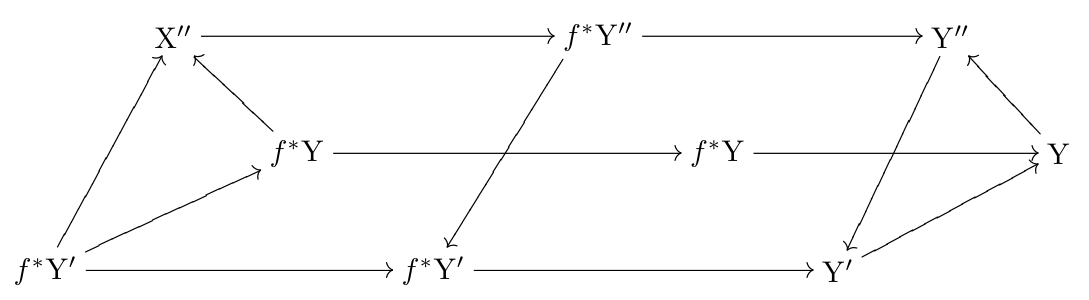
\includegraphics[width=.95\linewidth]{figures/sga4-3/diagram-2-2-13.png}
\]
证明 $s$ 为\Term{isomorphism}{同构}，即完成证明。对于 $\operatorname{Ob}\mathcal A_x$ 中任意 $X$，有\Term{commutative-diagram}{交换图}
\[
\resizebox{\linewidth}{!}{\begin{tikzcd}[ampersand replacement=\&,column sep=small]
\operatorname{Hom}_x(X,f^*Y')\arrow[r]\arrow[d,equal]\&\operatorname{Hom}_x(X,f^*Y)\arrow[r]\arrow[d,equal]\&\operatorname{Hom}_x(X,X'')\arrow[r]\arrow[d]\&\operatorname{Hom}_x(X,f^*Y'[1])\arrow[r]\arrow[d,equal]\&\operatorname{Hom}_x(X,f^*Y[1])\arrow[d,equal]\\
\operatorname{Hom}_x(X,f^*Y')\arrow[r]\arrow[d,equal]\&\operatorname{Hom}_x(X,f^*Y)\arrow[r]\arrow[d,equal]\&\operatorname{Hom}_x(X,f^*Y'')\arrow[r]\arrow[d,equal]\&\operatorname{Hom}_x(X,f^*Y'[1])\arrow[r]\arrow[d,equal]\&\operatorname{Hom}_x(X,f^*Y[1])\arrow[d,equal]\\
\operatorname{Hom}_f(X,Y)\arrow[r]\&\operatorname{Hom}_f(X,Y)\arrow[r]\&\operatorname{Hom}_f(X,Y'')\arrow[r]\&\operatorname{Hom}_f(X,Y'[1])\arrow[r]\&\operatorname{Hom}_f(X,Y[1]).
\end{tikzcd}}
\]
由 2.2.4，首行与末行\Term{exact-sequence}{正合}。由\Term{five-lemma}{五引理}，$s$ 诱导的从 $\operatorname{Hom}(X,X'')$ 到 $\operatorname{Hom}(X,f^*Y'')$ 的映射总是\Term{bijection}{双射}，因此 $s$ 为\Term{isomorphism}{同构}。
\end{proof}
对\Term{cofibered-category}{余纤维范畴}显然有\Term{duality}{对偶}结果。

\textbf{2.3。\Term{trivial-duality}{平凡对偶}公式。}设 $\mathcal A$ 为\Term{base-category}{基范畴} $\mathcal B$ 上的\Term{category}{范畴}，$S$ 为 $\mathcal A$ 的一组\Term{arrow}{箭头}，其中每个\Term{arrow}{箭头}都投到 $\mathcal B$ 的一个恒等\Term{arrow}{箭头}上。由\Term{calculus-of-fractions}{分式演算}从 $\mathcal A$ 得到的\Term{category}{范畴} $\mathcal A(S^{-1})$，是 $\mathcal B$ 上的一个\Term{category}{范畴}（由\Term{universal-property}{泛性质}）。

\SourcePage{191}
设 $\mathcal B'\to\mathcal B$ 为\Term{functor}{函子}；以 $\mathcal A'$ 表示\Term{fiber-product}{纤维积} $\mathcal A\times_{\mathcal B}\mathcal B'$，以 $S'$ 表示 $S$ 在 $\mathcal A'$ 中的\Term{inverse-image}{逆像}。复合\Term{functor}{函子} $\mathcal A'\to\mathcal A\to\mathcal A(S^{-1})$ 使 $S'$ 中的\Term{arrow}{箭头}\Term{invertible}{可逆}，因此通过 $\mathcal A'(S'^{-1})$ \Term{resolution}{分解}。这样得到\Term{canonical}{典范}的 $\mathcal B'$-\Term{functor}{函子}
\[
\mathcal A'(S'^{-1})\longrightarrow\mathcal B'\times_{\mathcal B}\mathcal A(S^{-1}).\tag{2.3.1}
\]

\begin{SGAresult}{引理}{2.3.2}
若 $\mathcal B'$ 是 $\mathcal B$ 的\Term{subcategory}{子范畴}，且每当 $\mathcal B$ 的复合\Term{arrow}{箭头} $h=f\circ g$ 属于 $\mathcal B'$ 时，$f$ 与 $g$ 也属于 $\mathcal B'$，则\Term{functor}{函子} (2.3.1) 是\Term{isomorphism}{同构}。
\end{SGAresult}
\begin{proof}
注意，(2.3.1) 总在\Term{object}{对象}上诱导\Term{bijection}{双射}，且在当前情形下，$\mathcal B'\times_{\mathcal B}\mathcal A(S^{-1})$ 是 $\mathcal A(S^{-1})$ 的\Term{subcategory}{子范畴}。

回顾 $\mathcal A(S^{-1})$ 的“显式”构造 [1，第 I 章]。给定 $\mathcal A$ 的两个\Term{object}{对象} $X,Y$，考虑“\Term{form}{形式}复合” $f_1\dots f_n$，每个 $f_i$ 或为 $\mathcal A$ 的\Term{arrow}{箭头}，或为 $S$ 中某个\Term{arrow}{箭头}的逆。\Term{set}{集合} $\operatorname{Hom}_{\mathcal A(S^{-1})}(X,Y)$ 是这些“\Term{form}{形式}复合”的\Term{set}{集合}模去由以下关系生成的\Term{equivalence-relation}{等价关系}所得的商：
\[
\begin{aligned}
f_1\dots uv\dots f_n&\equiv f_1\dots(u\circ v)\dots f_n&&u,v\in\operatorname{Fl}(\mathcal A),\\
f_1\dots ss^{-1}\dots f_n&\equiv f_1\dots f_n&&s\in S,\\
f_1\dots s^{-1}s\dots f_n&\equiv f_1\dots f_n&&s\in S.
\end{aligned}
\]
把这些构造用于 $\mathcal A$ 及其\Term{subcategory}{子范畴} $\mathcal A'$，即可验证 $\mathcal A'(S^{-1})$ 就是 $\mathcal A(S^{-1})$ 中 $\mathcal B'$ 的\Term{inverse-image}{逆像}\Term{subcategory}{子范畴}，因为如果一个“\Term{form}{形式}复合” $f_1\dots f_n$ 在 $\mathcal B$ 中的复合是 $\mathcal B'$ 的\Term{arrow}{箭头}，则每个 $f_i$ 的像也都是 $\mathcal B'$ 的\Term{arrow}{箭头}。
\end{proof}
现在假定 $\mathcal A$ 是 $\mathcal B$ 上的\Term{triangulated-category}{三角范畴}，且对 $x\in\operatorname{Ob}(\mathcal B)$，\Term{set}{集合} $S_x=S\cap\operatorname{Fl}(\mathcal A_x)$ 都是\Term{saturated-multiplicative-system}{饱和乘法系}（CD 第 I 章第 2 节 1）。

\begin{SGAresult}{定义}{2.3.3}
在上述假设下，如果对每个\Term{functor}{函子} $F:\mathcal B'\to\mathcal B$，\Term{functor}{函子} (2.3.1) 都是\Term{isomorphism}{同构}，则称\Term{category}{范畴} $\mathcal A/\mathcal B$ 相对于 $S$ \Term{almost-derivable}{几乎可导出}；若此外 $\mathcal A(S^{-1})$ 在 $\mathcal B$ 上\Term{fibered-category}{纤维化}（相应地，\Term{cofibered-category}{余纤维化}），则称它相对于 $S$ \Term{derivable-category}{可导出}（相应地，\Term{coderivable-category}{余可导出}）。
\end{SGAresult}
以 $I$ 表示下图的\Term{category}{范畴}：
\[
I:\quad X_0\xrightarrow{F}X_1.\tag{2.3.4}
\]
由 2.2.13，给定 $I$ 上的一个\Term{triangulated-category}{三角范畴} $\mathcal A$，它在 $\mathcal A$ 上\Term{fibered-category}{纤维化}（相应地，\Term{cofibered-category}{余纤维化}），\Term{equivalence}{等价}于给定其\Term{fiber}{纤维} $\mathcal A_0$ 与 $\mathcal A_1$，以及\Term{triangulated-functor}{三角}\Term{inverse-image}{逆像}\Term{functor}{函子}
\SourcePage{192}
$F^*:\mathcal A_1\to\mathcal A_0$（相应地，\Term{triangulated-functor}{三角}\Term{direct-image}{直接像}\Term{functor}{函子} $F_*:\mathcal A_0\to\mathcal A_1$）。若 $A_0\in\operatorname{Ob}\mathcal A_0$、$A_1\in\operatorname{Ob}\mathcal A_1$，则有（2.2.12.1）
\[
\operatorname{Hom}_F(A_0,A_1)=\operatorname{Hom}(A_0,F^*A_1)
\]
（相应地，$\operatorname{Hom}_F(A_0,A_1)=\operatorname{Hom}(F_*A_0,A_1)$）。

\begin{SGAresult}{命题}{2.3.5}
设 $\mathcal A$ 为 $I$ 上的\Term{triangulated-category}{三角范畴}，$S$ 如 2.3.3。
\begin{enumerate}
\item[(i)] $\mathcal A$ 相对于 $S$ \Term{almost-derivable}{几乎可导出}，且 $\mathcal A(S^{-1})$ 是 $I$ 上的\Term{triangulated-category}{三角范畴}。
\item[(ii)] 若 $\mathcal A$ \Term{fibered-category}{纤维化}（相应地，\Term{cofibered-category}{余纤维化}），则\Term{functor}{函子} $F^*$（相应地，$F_*$）相对于 $S_0$、$S_1$ \Term{right-derivable}{右可导出}（相应地，\Term{left-derivable}{左可导出}）（1.2.1），当且仅当 $\mathcal A$ 在 $I$ 上\Term{derivable-category}{可导出}（相应地，\Term{coderivable-category}{余可导出}）。
\end{enumerate}
\end{SGAresult}
\begin{proof}
由 2.3.2，$\mathcal A(S^{-1})$ 的\Term{fiber-category}{纤维范畴}为 $\mathcal A_0(S_0^{-1})$、$\mathcal A_1(S_1^{-1})$，其中 $S_i=S\cap\operatorname{Fl}(\mathcal A_i)$（$i=0,1$）。沿用第 1 节第 2 小节的记号，\Term{functor}{函子} $A_0\mapsto A_0^-$ 与 $A_1\mapsto A_1^+$ 把 $\mathcal A_0(S_0^{-1})$ 与 $\mathcal A_1(S_1^{-1})$ 分别等同于 $\mathcal A_0$、$\mathcal A_1$ 的\Term{pro-object}{pro-对象}与\Term{ind-object}{ind-对象}所成的\Term{category}{范畴}。由此可以定义 $I$ 上的一个\Term{category}{范畴}，\Term{fiber}{纤维}为 $\mathcal A_0(S_0^{-1})$、$\mathcal A_1(S_1^{-1})$：对 $A_0\in\mathcal A_0$、$A_1\in\mathcal A_1$，置
\[
\operatorname{Hom}_F(A_0,A_1)=\operatorname{Hom}_F(A_0^-,A_1^+)
=\varinjlim_{A'_0\xrightarrow{s}A_0}\ \varinjlim_{A_1\xrightarrow{t}A'_1}\operatorname{Hom}(A'_0,A'_1),
\]
其中 $s$、$t$ 遍历 $S_0$、$S_1$ 中以 $A_0$ 为靶、以 $A_1$ 为源的元素。\Term{category}{范畴} $\mathcal A$ 映到这个\Term{category}{范畴}中；立即可以验证，在 $I$ 上以及任意\Term{base-change}{基变换}后，它都满足 $\mathcal A(S^{-1})$ 的\Term{universal-property}{泛性质}。

为验证 (i)，只须证明这个\Term{category}{范畴}，即 $\mathcal A(S^{-1})$，是\Term{triangulated-category}{三角范畴}；而只须验证条件 2.2.3 (iii)。因此设 $(X_0,Y_0,Z_0)$ 与 $(X_1,Y_1,Z_1)$ 分别为 $\mathcal A_0$、$\mathcal A_1$ 的\Term{distinguished-triangle}{区别三角}，在 $\mathcal A_0(S_0^{-1})$、$\mathcal A_1(S_1^{-1})$ 中给出\Term{distinguished-triangle}{区别三角} $(X_0^-,Y_0^-,Z_0^-)$ 与 $(X_1^+,Y_1^+,Z_1^+)$，并给定图
\[
\begin{tikzcd}
X_0^-\arrow[r,"u"]\arrow[d]&X_1^+\arrow[d]\\
Y_0^-\arrow[r,"v"']&Y_1^+.
\end{tikzcd}\tag{2.3.5.1}
\]
由引理 1.2.2.1，三角 $(X_0^-,Y_0^-,Z_0^-)$ 与 $(X_1^+,Y_1^+,Z_1^+)$ 是\Term{distinguished-triangle}{区别三角}的\Term{limit}{极限}；因而存在\Term{distinguished-triangle}{区别三角}的\Term{morphism}{态射}
\[
\begin{aligned}
(X_0^-,Y_0^-,Z_0^-)&\longrightarrow(X'_0,Y'_0,Z'_0),\\
(X'_1,Y'_1,Z'_1)&\longrightarrow(X_1^+,Y_1^+,Z_1^+),
\end{aligned}\tag{2.3.5.2}
\]
以及与 (2.3.5.1) 相容的图
\SourcePage{193}
\[
\begin{tikzcd}
X'_0\arrow[r,"u'"]\arrow[d]&X'_1\arrow[d]\\
Y'_0\arrow[r,"v'"']&Y'_1.
\end{tikzcd}
\]
由于\Term{category}{范畴} $\mathcal A$ 在 $I$ 上是\Term{triangulated-category}{三角范畴}，此图可延拓成三角\Term{morphism}{态射}
\[
(X'_0,Y'_0,Z'_0)\longrightarrow(X'_1,Y'_1,Z'_1).
\]
将它与\Term{morphism}{态射} (2.3.5.2) 复合，就看出图 (2.3.5.1) 可以延拓成三角\Term{morphism}{态射}，从而证明了 2.2.3 (iii)。

验证 (ii)，例如假定 $\mathcal A$ 在 $I$ 上\Term{fibered-category}{纤维化}。若 $A_1\in\operatorname{Ob}(\mathcal A_1(S_1^{-1}))$，则 $A_1$ 在 $\mathcal A(S^{-1})$ 中的一个\Term{inverse-image}{逆像}，是 $\mathcal A_0(S_0^{-1})$ 的\Term{object}{对象} $B$，使在 $\mathcal A_0(S_0^{-1})$ 中有
\[
\begin{aligned}
\operatorname{Hom}_{\mathcal A_0(S_0^{-1})}(A_0,B)
&=\operatorname{Hom}_F(A_0^-,A_1^+)=\operatorname{Hom}(A_0^-,F^*(A_1^+))\\
&=\operatorname{Hom}_{\mathcal A_0(S_0^{-1})}(A_0,F^*(A_1^+)).
\end{aligned}
\]
这样的\Term{object}{对象} $B$ 存在，当且仅当 $\mathcal A_0(S_0^{-1})$ 的\Term{ind-object}{ind-对象} $F^*(A_1^+)$ \Term{essentially-constant-ind-object}{本质常值}（即\Term{representable}{可表}）；此时 $B$ 表示这个\Term{ind-object}{ind-对象}，而它正是 $RF(A_1)$（1.2.1），故得所断。
\end{proof}

\begin{SGAresult}{推论}{2.3.6}
沿用 2.3.3 的记号，若 $\mathcal A$ 在 $\mathcal B$ 上\Term{almost-derivable}{几乎可导出}，则 $\mathcal A(S^{-1})$ 是 $\mathcal B$ 上的\Term{triangulated-category}{三角范畴}。
\end{SGAresult}
\begin{proof}
首先，\Term{fiber-category}{纤维范畴} $\mathcal A(S^{-1})_x$ 可等同于 $\mathcal A_x(S_x^{-1})$：把假设用于\Term{base-change}{基变换} $\{x\}\to\mathcal B$ 即可。这是一个配备三角\Term{set}{集合} $\Delta_x$ 的\Term{triangulated-category}{三角范畴}，于是上述命题有了意义。为验证条件 2.2.3 (iii)，只须在每个\Term{base-change}{基变换} $I\to\mathcal B$ 后验证；所断即由 2.3.5 (i) 得到。
\end{proof}
由 2.3.5 (ii) 的证明立即得到：

\begin{SGAresult}{定理}{2.3.7（\Term{trivial-duality}{平凡对偶}公式）}
设 $\mathcal A$ 是 $I$ 上\Term{fibered-category}{纤维化}且\Term{cofibered-category}{余纤维化}的\Term{triangulated-category}{三角范畴}，以 $F_*$、$F^*$ 分别表示\Term{direct-image}{直接像}和\Term{inverse-image}{逆像}\Term{functor}{函子}。设 $S=S_0\cup S_1$ 为 2.3.3 中的\Term{multiplicative-system}{乘法系}。假定 $LF_*$ 在 $A_0\in\operatorname{Ob}\mathcal A_0(S_0^{-1})$ 处有定义，$RF^*$ 在 $A_1\in\operatorname{Ob}\mathcal A_1(S_1^{-1})$ 处有定义。那么
\[
\operatorname{Hom}_{\mathcal A_0(S_0^{-1})}(A_0,RF^*A_1)
=\operatorname{Hom}_{\mathcal A(S^{-1})}(A_0,A_1)
=\operatorname{Hom}_{\mathcal A_1(S_1^{-1})}(LF_*A_0,A_1).
\]
\end{SGAresult}
2.3.7 中\Term{signature}{符号} $R$、$L$、$*$ 及 ${}^*$ 的位置只是看起来反常；事实上，在 0.2 的变动\Term{site}{景}上的\Term{sheaf}{层}所成的\Term{fibered-category}{纤维范畴}兼\Term{cofibered-category}{余纤维范畴}中，\Term{fiber-category}{纤维范畴}是通常\Term{sheaf}{层}\Term{category}{范畴}的\Term{opposite-category}{反范畴}。
\SourcePage{194}
\textbf{2.4。以\Term{derived-category}{导出范畴}为\Term{fiber}{纤维}的\Term{category}{范畴}。}

\textbf{2.4.0。}本小节以 $\mathcal A$ 表示 $\mathcal B$ 上的一个\Term{cofibered-category}{余纤维化}\Term{triangulated-category}{三角范畴}，$S$ 表示 $\mathcal A$ 的\Term{morphism}{态射}的一个\Term{multiplicative-system}{乘法系}，其中每个\Term{morphism}{态射}都位于一个恒等\Term{arrow}{箭头}之上，且对于每个 $x\in\operatorname{Ob}(\mathcal B)$，$S_x=S\cap\operatorname{Fl}(\mathcal A_x)$ 是 $\mathcal A_x$ 的\Term{saturated-multiplicative-system}{饱和乘法系} [CD 1.2.1]。

我们寻找 $\mathcal A$ 相对于 $S$ \Term{coderivable-category}{余可导出}（2.3.3）的一个判据；这将推出，把与 $\mathcal A$ 的\Term{distinguished-triangle}{区别三角}的像\Term{isomorphism}{同构}的三角组成\Term{set}{集合}，配给 $\mathcal A(S^{-1})$ 后，$\mathcal A(S^{-1})$ 是 $\mathcal B$ 上的\Term{triangulated-category}{三角范畴}（2.3.5）。

\begin{SGAresult}{命题}{2.4.1}
设 $\mathcal A$、$\mathcal B$、$S$ 如上。为使 $\mathcal A$ 相对于 $S$ \Term{coderivable-category}{余可导出}，下述条件成立即已足够：
\[
\begin{gathered}
(*)\quad\forall x\in\operatorname{Ob}\mathcal B,\quad\forall A\in\operatorname{Ob}(\mathcal A_x),\quad\exists s:A'\to A\text{ 属于 }S,\\
\forall g,f:x\xrightarrow{f}y\xrightarrow{g}Z,\quad
f_*A'\text{ 对函子 }g_*\text{ 左适配}.
\end{gathered}
\]
\end{SGAresult}
以 $\mathcal A^1$ 表示 $\mathcal A$ 的一个\Term{full-subcategory}{满子范畴}，其\Term{object}{对象}的所有\Term{direct-image}{直接像}相对于所有\Term{direct-image}{直接像}\Term{functor}{函子}均\Term{derived-adapted}{适配}。由 1.2.2，$\mathcal A^1$ 是 $\mathcal A$ 的\Term{triangulated-subcategory}{三角子范畴}，且显然\Term{cofibered-category}{余纤维化}。置 $S^1=S\cap\operatorname{Fl}(\mathcal A^1)$。

\begin{SGAresult}{引理}{2.4.1.1}
假定 $S$ 在\Term{direct-image}{直接像}下\Term{stable}{稳定}。那么 $\mathcal A/\mathcal B$ \Term{coderivable-category}{余可导出}，且 $\mathcal A(S^{-1})$ 可由右\Term{calculus-of-fractions}{分式演算}算出。
\end{SGAresult}
\begin{proof}
来验证 [1, I 2.2] 的条件 c)，它或许不像其他条件那么平凡。给定 $f$ 与 $s$（$s\in S$），须找到一个 $t\in S$ 的\Term{commutative-diagram}{交换图}
\[
\begin{tikzcd}
A'\arrow[r,dashed]&B'\\
A\arrow[u,"s"]\arrow[r,"f"']&B\arrow[u,dashed,"t"'].
\end{tikzcd}\tag{2.4.1.2}
\]
设 $F$ 为 $f$ 在 $\mathcal B$ 中的像。由假设，$F_*(s)$ 仍属于 $S$，故由 Verdier 的结果，存在\Term{commutative-diagram}{交换图}
\[
\begin{tikzcd}
F_*(A')\arrow[r]&B'\\
F_*(A)\arrow[u,"s"]\arrow[r,"f"']&B\arrow[u,"t"'].
\end{tikzcd}
\]
于是也有一个图 (2.4.1.2)。

由于 $\mathcal A(S^{-1})$ 可用右\Term{calculus-of-fractions}{分式演算}计算，其形成与\Term{base-change}{基变换} $c:\mathcal B'\to\mathcal B$ 交换是平凡的。
\end{proof}
\SourcePage{195}
此引理特别适用于 $\mathcal A^1$ 与 $S^1$；因此下述引理推出 2.4.1。

\begin{SGAresult}{引理}{2.4.1.3}
在 $\mathcal B$ 上以及任意\Term{base-change}{基变换} $c:\mathcal B'\to\mathcal B$ 后，\Term{canonical}{典范}\Term{functor}{函子} $\Phi:\mathcal A^1(S^{1-1})\to\mathcal A(S^{-1})$ 都是\Term{equivalence-of-categories}{范畴等价}。
\end{SGAresult}
\begin{proof}
来构造\Term{functor}{函子} $\Phi$ 的一个\Term{quasi-inverse}{拟逆}。对任意 $A\in\operatorname{Ob}\mathcal A$，选取 $s_A\in S$，以 $A$ 为靶、以 $A^1\in\operatorname{Ob}\mathcal A^1$ 为源，并在 $A\in\operatorname{Ob}\mathcal A^1$ 时令 $s_A=\operatorname{Id}_A$。设 $f$ 为 $\mathcal A$ 的一个\Term{arrow}{箭头}，以 $A$ 为靶，以 $B$ 为源，在 $\mathcal B$ 中的像为 $F$。由于 $s_B\in S$ 且 $F_*A^1\in\operatorname{Ob}\mathcal A^1$，可以找到 $B^1$、$u$ 及 $s\in S^1$，使下图交换：
\[
\begin{tikzcd}[column sep=large,row sep=large]
A\arrow[r,"f"]&B\arrow[r,"s_B"]&B^1\\
A^1\arrow[u,"s_A"]\arrow[r,"a"']&F_*A^1\arrow[u]&B'\arrow[l,"s"]\arrow[u,"u"'].
\end{tikzcd}\tag{2.4.1.4}
\]
于是，$\mathcal A^1(S^{1-1})$ 的\Term{arrow}{箭头} $f^1=us^{-1}a$ 只依赖于 $f$。

设 $f,g$ 是两个可复合的\Term{arrow}{箭头}，其在 $\mathcal B$ 中的像为 $F,G$。为证明 $(g\circ f)^1=g^1\circ f^1$，考察下图，其中包含 $f$ 与 $g$ 的 (2.4.1.4) 型图：
\[
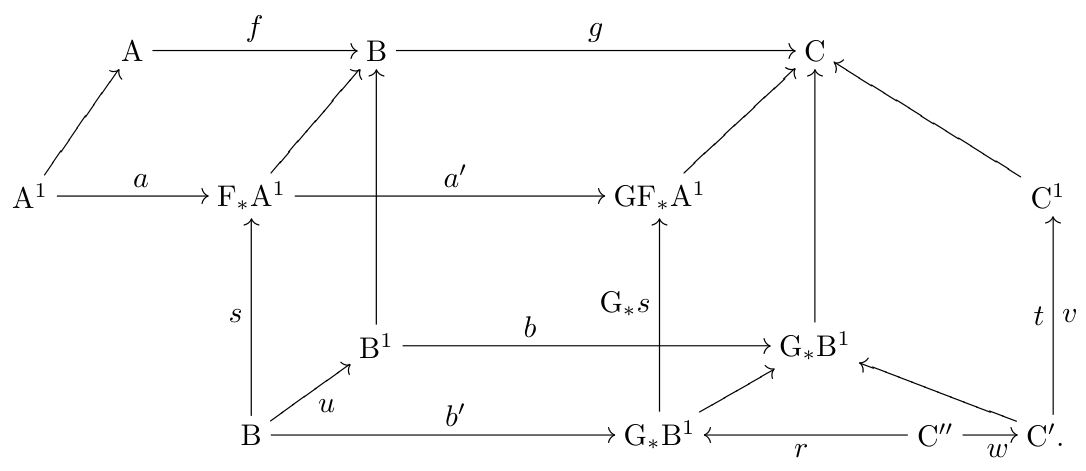
\includegraphics[width=.97\linewidth]{figures/sga4-3/diagram-2-4-1-composition.png}
\]
因为 $t\in S$，存在 $C''$、$r\in S^1$ 及 $w$ 使该图交换。按定义，
\[
g^1\circ f^1=vt^{-1}bus^{-1}a,\qquad
(g\circ f)^1=vw(G_*(s)r)^{-1}a'a;
\]
由图的交换性即得结论。

这样定义了一个从 $\mathcal A$ 到 $\mathcal A^1(S^{1-1})$ 的\Term{functor}{函子}；由 $\mathcal A(S^{-1})$ 的\Term{universal-property}{泛性质}，它\Term{resolution}{分解}为 $\Psi:\mathcal A(S^{-1})\to\mathcal A^1(S^{1-1})$。复合 $\Phi\Psi$ \Term{isomorphism}{同构}于恒等\Term{functor}{函子}，因为它与\Term{functor}{函子} $J:\mathcal A\to\mathcal A(S^{-1})$ 的复合\Term{isomorphism}{同构}于 $J$。同样可以验证 $\Psi\Phi$ \Term{isomorphism}{同构}于恒等\Term{functor}{函子}。
\end{proof}

\SourcePage{196}
\begin{SGAresult}{推论}{2.4.2}
沿用 2.4.1 的记号，只要对于 $\mathcal B$ 中的每个\Term{finite}{有限}\Term{arrow}{箭头}集 $B$，把条件 $(*)$ 中所考虑的\Term{direct-image}{直接像}\Term{restriction}{限制}为沿 $B$ 中\Term{arrow}{箭头}取\Term{direct-image}{直接像}时，条件 $(*)$ 成立，则 $\mathcal A$ 相对于 $S$ \Term{coderivable-category}{余可导出}。
\end{SGAresult}
\begin{proof}
对于任意\Term{arrow}{箭头}集\Term{finite}{有限}的\Term{category}{范畴} $\mathcal B'$，每次\Term{base-category}{基范畴}变换 $\mathcal B'\to\mathcal B$ 后，命题 2.4.1 都适用。取 $\mathcal B'$ 为下列各图的\Term{category}{范畴}：
\[
\begin{array}{cccc}
* & *\longrightarrow * & *\longrightarrow *\longrightarrow * & *\longrightarrow *\longrightarrow *\longrightarrow *\\[1ex]
(0)&(1)&(2)&(3).
\end{array}
\]
考虑\Term{category}{范畴} $\mathcal A_x(S_x^{-1})$（$x\in\operatorname{Ob}\mathcal B$）。给定 $f\in\operatorname{Fl}(\mathcal B)$，以及这些\Term{category}{范畴}中分别位于 $f$ 的源、靶之上的 $A_1,A_2$，把 $\operatorname{Hom}_f(A_1,A_2)$ 定义为沿 $f$ 所定义的 (1) 型\Term{base-category}{基范畴}变换后得到的相应\Term{set}{集合}。利用 (3) 型\Term{base-category}{基范畴}变换定义\Term{morphism}{态射}的复合。如此构造出 $\mathcal B$ 上的一个\Term{category}{范畴} $\mathcal A(S^{-1})^*$，其形成与任意\Term{base-change}{基变换}相容；利用 (0)、(1)、(2) 型\Term{base-category}{基范畴}变换，可以验证它是定义 $\mathcal A(S^{-1})$ 的\Term{universal-property}{泛问题}的解。
\end{proof}
下述结果是 2.4.2 的\Term{duality}{对偶}。

\begin{SGAresult}{命题}{2.4.3}
设 $\mathcal A$ 是 $\mathcal B$ 上\Term{fibered-category}{纤维化}的\Term{triangulated-category}{三角范畴}，$S$ 如 2.4.1。为使 $\mathcal A$ 相对于 $S$ \Term{derivable-category}{可导出}，只须对 $\mathcal B$ 的每个\Term{finite}{有限}\Term{arrow}{箭头}集 $B$，有
\[
\begin{gathered}
(*')\quad\forall x\in\operatorname{Ob}(\mathcal B),\quad\forall A\in\operatorname{Ob}(\mathcal A_x),\quad\exists s:A\to A'\text{ 属于 }S,\\
\forall g,f:Z\xrightarrow{g}Y\xrightarrow{f}X\text{ 属于 }B,\quad
f^*A'\text{ 对函子 }g^*\text{ 右适配}.
\end{gathered}
\]
\end{SGAresult}
